%!TEX root=../tax-democracy-held.tex

\chapter[Tax Matters]{Why Tax Matters to the Welfare State} \label{chap:tax-matters}

\begin{quote}
	\emph{``The spirit of a people, its cultural level, its societal structure, the deeds its policy may prepare --- all this and more is written in its fiscal history, stripped of all phrases. He who knows how to listen to its message here discerns the thunder of world history more clearly than anywhere else''.}\\*
	--- Joseph Schumpeter (1918 [1991])
\end{quote}

%note from new yorker article how jk galbraith said that the rich should erect a statue to the PIT, because it allows great income inequality. Note to that that things might have changed today

%Some introduction of why tax matters, what this thesis looks at.

	% it is by the states capacity to reallocate market equivalent incomes that the welfare retrenchment should be all about, and that is: reallocation WITHOUT debt of one form or another. Important: a welfare retrenchment test should be independent of how market outcomes are reallocated, be it through taxation, or whatever.
		%Hunch: welfare state is worse today.

\section{Why it Matters: The Welfare State as Mixed Economy} \label{sec:why-mixed-economy-matters}

\begin{quote}
	\emph{``Yes we can: to justice and equality.\\ Yes we can: to opportunity and prosperity.''\\}
	--- Barack H. Obama, Obama For America 2008
\end{quote} %better quote, anyone?

%Moreover, economists like Nicholas Barr (20013, 2004) argue that social insurance programs step in where markets fail. Given (via Mau/Leibfried)

%this is a better, more systematic way to think about problems and welfare, otherwise we're just confused.

At this point, a reader may ask: why would all, or even any of this, matter to the welfare state?

Materially possible and normatively desirable welfare states are, and must be thought of as, well-designed mixed economies, for at least three reasons:

\begin{enumerate}
	\item \emph{Engaging Complexity.} In a welfare state, \hyperref[sec:interface]{exchange and command modes of production and distribution, inevitably, complexly interact and easily produce unintended consequences} (p.~\pageref{sec:interface}). For example, a \hyperref[sec:prince-controls]{minimum wage may cause structural unemployment} (p.~\pageref{sec:price-controls}) and the \hyperref[sec:well-determined-incidence]{\emph{nominal} incidence of a tax will be entirely inconsequential} (p.~\pageref{sec:well-determined-incidence}). 
	
	To eradicate today, as Lord Beveridge promised 150 years ago, the five `Giant Evils' of want, disease, ignorance, squalor and idleness, you have to anticipate this interplay of market and government and choose accordingly. The mixed economy provides us with a toolset to analyze the complexity of welfare states, including the dynamics presented here. For example, the mixed economy suggests we should always check the \gls{DWL} (p.~\pageref{sec:minimal-DWL}) and \hyperref[sec:well-determined-incidence]{incidence} (p.~\pageref{sec:well-determined-incidence}) of any redistribution, a welfare state may undertake.
	
	To answer the first-order question of welfare state design, as I have here tried to do, we need the abstractions of the mixed economy to know what is \emph{materially possible} in a scarce world, filled with (at least some) homines oeconomici. For example, price controls may not be possible (without grave losses), but a well-designed, personal, almost arbitrarily progressive taxation \emph{is} indeed possible in a closed economy.	
	
	\item \emph{Denaturalizing Market Allocations.} When we consider welfare state programs in isolation from the markets which they supplant, we easily end up naturalizing whatever markets have allocated. In fact, any given market exchange which a welfare state may seek to correct, is already and always \emph{contingent} on the institutions, dynamics and distributions under which it occured. 
	
	For example, rather than ``fighting poverty'' --- as if that were an objective reality --- welfare states must consider overall allocative dynamics (such as \hyperref[sec:winner-take-all]{winner-take-all}, p.~\pageref{sec:winner-take-all}) and distributions (such as \hyperref[sec:monopsony-employers]{monopsony employers}, p.~\pageref{sec:monopsony-employers}), and counteract them, as is seen fair. Markets do not make some people below an arbitrarily defined threshold ``poor'', and leave others ok or even untouched. Instead, markets allocate incomes across the \emph{entire} spectrum contingent on a host of institutions, dynamics and initial distributions. If government pursues a particular minimum standard of living for everyone, it might not only transfer income to those who fall below it, but may need to counteract those dynamics under which people slipped below the minimum standard in the first place. 
	
	Market allocations, in short, are --- and should be --- no less subject to enlightened, collective human choice than remedial welfare state programs: ``Increasing dependency is no law of nature but the result of socio-economic changes, which in turn react to human intervention'' (\citealt{Esping-Andersen2002}: x).
	
	\item \emph{Caring about Outcomes.} \citeauthor{Haggard2009} (\citeyear[236]{Haggard2009}) remind us about
		\begin{quote}
			``(\ldots) the importance of pushing the research on the [Eastern European] welfare state down the causal chain towards its social consequences. (\ldots) [A]ny meaningful strategy of comparison of the welfare state must ultimately engage its consequences for a variety of outcomes, from poverty and inequality, to physical quality of life measures, to economic outcomes such as the efficiency of labour markets, competitiveness and even economic growth. In the first instance, we are interested in the welfare state because we are interested in human welfare.''
		\end{quote}
	
	The abstractions of the mixed economy I have summarized here synthesize a lot of what we need to know about the material, and therefore social consequences of a capitalist welfare state. 

	When we care about social consequences, the mixed economy suggests a great deal more to consider than just nominal welfare programs. For example, welfare states should not only provide social insurance, but also redress failing \hyperref[sec:public-good]{public goods} (p.~\pageref{sec:public-good}) and \hyperref[sec:long-term-inconsistency]{make us save enough for our children} (p.~\pageref{sec:long-term-inconsistency}). 
	
	When we care about social consequences, the mixed economy also implies that not all welfare programs are created equal. For example, welfare states interventions should \hyperref[sec:minimal-DWL]{distort market prices as little as possible} (p.~\pageref{sec:minimal-DWL}) and use \hyperref[sec:price-stability]{monetary expansion only sparingly, for short-term stimulus} (p.~\pageref{sec:price-stability}).
	
	When we care about social consequences, the mixed economy suggests that  governments and markets are better at different things, and it ties welfare state interventions to specific justifications. For example, welfare states should nationalize or regulate utility markets if and to the extent that they are \hyperref[sec:natural-monopoly]{natural monopolies} (p.~\pageref{sec:natural-monopoly}), but there is no reason to (as Germany presently does) redistribute within \hyperref[sec:state-insurance]{social health insurance} (p.~\pageref{sec:state-insurance}), who was supposed to only save the risk pool from \hyperref[sec:adverse-selection]{adverse selection} (p.~\pageref{sec:adverse-selection}). Caring about social consequences also means to leave markets alone, if they will likely serve material human need best.
	
	When we care about social consequences, the mixed economy reveals that efficiency and equity are not always opposed, but often go hand in hand. 
	\begin{enumerate}
		\item \emph{Inefficient is Inequitable.} \citeauthor{Titmuss1974} urged welfare states not to exclusively concentrate on poverty relief because such ``residual services (\ldots) often become poor services for poor people'' (\citeyear{Titmuss1974}: 134). This intuition is supported by the abstractions of the mixed economy: as the rich are forced or allowed to take the inefficient --- but for them, affordable --- exit route from government provision, a retrenched welfare state will offer only inferior provision, or none at all, to those too poor to exit. 
		
		This problem is particularly acute in health or disability insurance: as the rich and healthy exit the risk pool, coverage becomes ever more expensive, driving even more people out until it \hyperref[sec:adverse-selection]{fails} (p.~\pageref{sec:adverse-selection}). 
		
		Similar distributive effects occur in a wider class of market failures, too. For example, a failed \hyperref[sec:common-good]{commons} (p.~\pageref{sec:common-good}) of global climate or local public safety will not only be wastefully inefficient, but it will also hit hardest the poorest regions and people, who can least afford substitutes, such as building a levee or hiring private protection. 
		
		\item \emph{Inequitable is Inefficient.} On the other hand, the abstractions of the mixed economy also imply that sometimes, slicing the pie unequally, will also make it smaller: ``(\ldots) there is a very good argument that equality of opportunities and life chances is becoming sine qua non for efficiency as well'' (\citealt{Esping-Andersen2002}: ix).
		
		For example, people may not be able to align the \hyperref[sec:principal-agent-problem]{interests of principals and agents} when collateral is not widely available (p.~\pageref{sec:principal-agent-problem}), and overly taxing low and middle (labor) incomes may contribute to \hyperref[sec:minimal-DWL]{structural unemployment} (p.~\pageref{sec:minimal-DWL}).
	\end{enumerate}
	
	To answer the first-order question of welfare state design, as I have here tried to do, we need the abstractions of the mixed economy to know what is \emph{normatively desirable} in a scarce world, filled with (at least some) homines oeconomici.	
\end{enumerate}

\paragraph[Higher Equilibria]{Higher Equilibria.} The first-order conflict about the best, possible welfare state is about the trade-offs, contradictions and uncertainties of the mixed economy explained in the above. My aim here was not to resolve that conflict: we may not know for sure, let alone agree on what \emph{the best} welfare state looks like (even though I offered some well-informed hunches). A mixed economy can --- in principle and for my purposes here --- make \emph{arbitrary} trade-offs between equity and efficiency, presence and future, or any of the other dimensions of human material need. 

	%3) There are inevitable contradictions in todays political economy of fighting the dynamics of inequality which the welfare state is systematically, (one wonders: on purpose?) ill-equipped to adress. (think income taxation)

But given \emph{any} preference set for these (sometimes!) competing goals, there are still more and less efficient institutional configurations for the mixed economy. More efficient, in this broadest sense, means that these configurations achieve more on \emph{all} goals. These preferable mixed economies will still trade off preferred goals for less preferred goals, but the trade-off will be less harsh. For example, a \gls{NIT} may achieve the same, if not more equity than a minimum wage, but at much lower cost in growth, or unemployment. Of course, you still have to break eggs for the proverbial omelette, just fewer of them.

% here used to be \ref{fig:ppf-values}, which is now gone only in wanted.

%DUPLICATE!!!%
\begin{figure}[htbp]
	\centering
	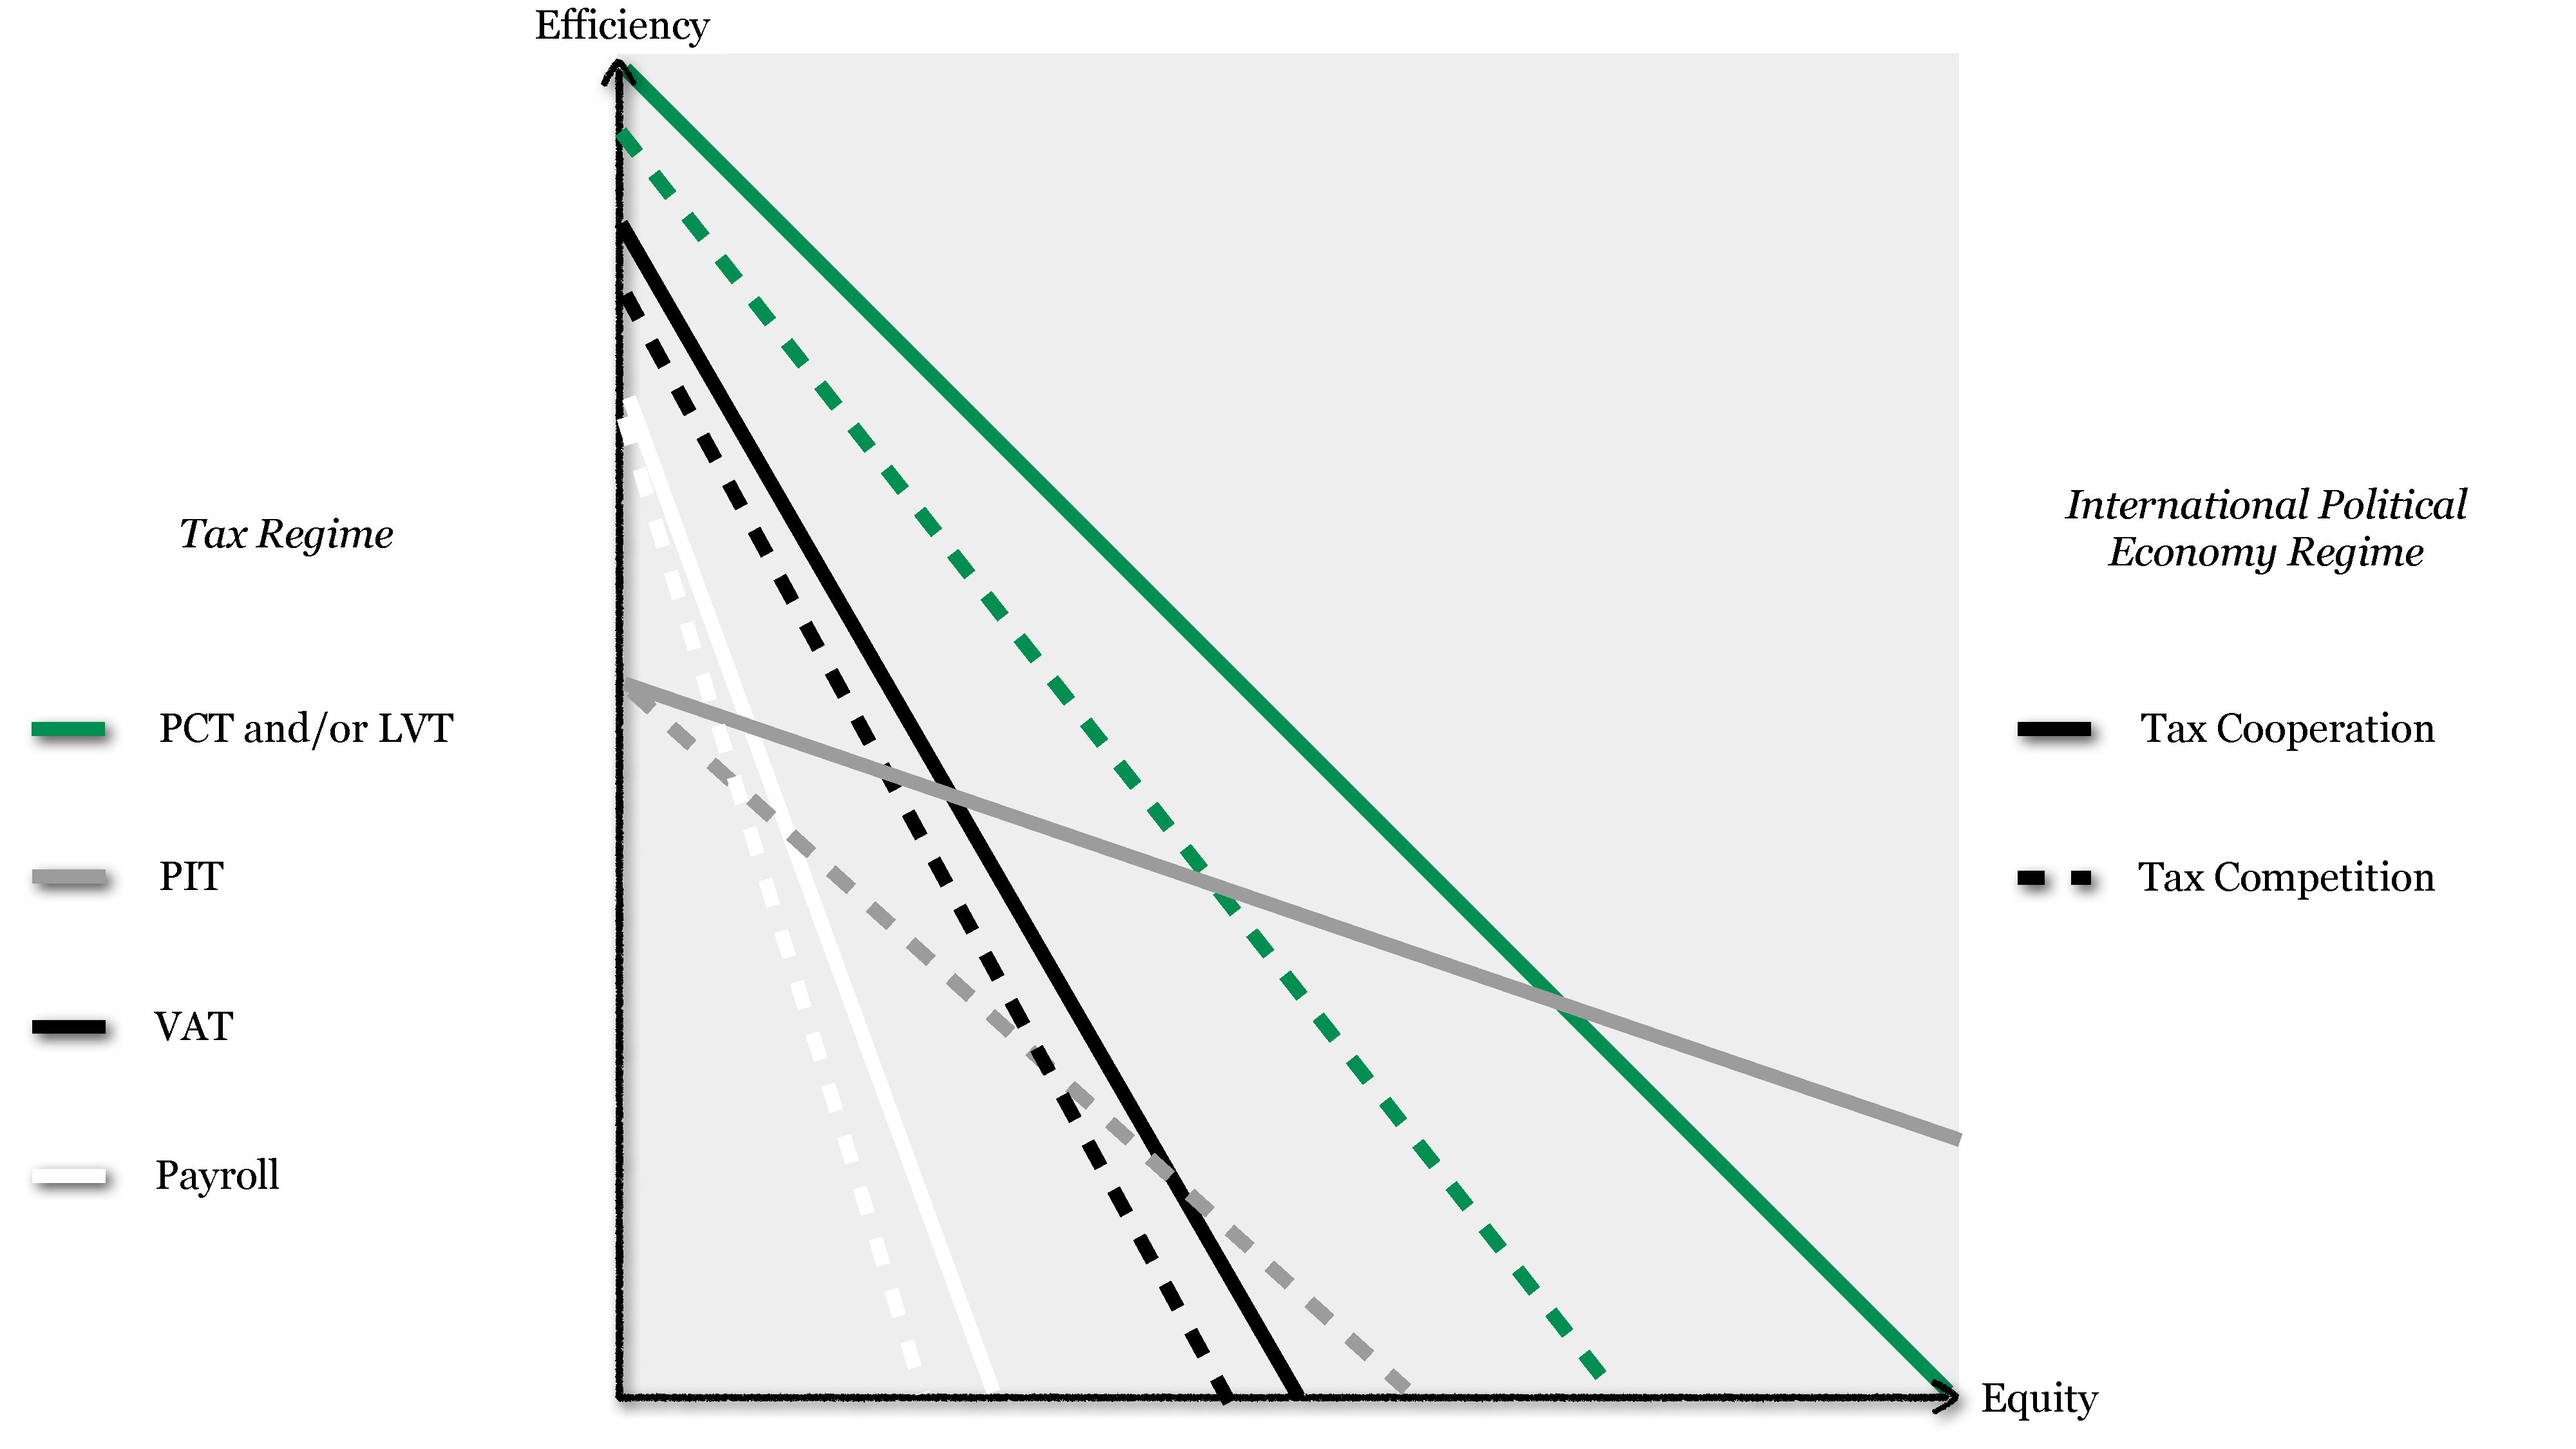
\includegraphics[width=1\linewidth]{ppf-tax-regimes}  
	\caption[Equity-Efficiency Trade-offs of Different Tax Regimes]{A Production Possibilities Frontier of Equity and Efficiency in Different Tax Regimes}
	\label{fig:ppf-tax-regimes} %add compare footnote to \ref{fig:ppf-values}
\end{figure}

The competing goals of human material need, in other words, are not always in a pure and immutable zero-sum relation, where, for example, one increment more in equity means one less in efficiency, one more in present consumption one less in future consumption. Depending on the institutional design, these conversion rates will differ: sometimes, for example, one increment in equity will cost only a half-increment in efficiency. Alternative mixed economies, more often than not, are a positive or --- equivalently --- negative sum proposition. 

Just entering the preferences between purposely competing goals does \emph{not} yield a single configured mixed economy, but many different blends of command and exchange production and distribution. Again, we may not know or agree what the globally optimal configuration is, given our preferences, but checking \hyperref[sec:means]{means} and \hyperref[sec:ends]{ends} of a mixed economy, we \emph{can} know better from worse configurations, or local optima.

A better welfare state is that mixed economy which elegantly combines \hyperref[sec:command]{command} and \hyperref[sec:exchange]{exchange} components to \hyperref[sec:production]{produce efficiently}, \hyperref[sec:risk]{pool risks}, \hyperref[sec:distribution]{distribute equitably}, \hyperref[sec:time]{consistent over time} and \hyperref[sec:space]{convergent over space}. That is, a welfare state that offers one of the higher possible trade-offs of growth, individual security, equality, saving and convergence. It does so without effectively borrowing from the future through \hyperref[sec:smoke-n-mirrors]{smoke and mirrors}, or hidden, but \hyperref[sec:real-dissavings]{real dissavings}. 

%Do I need the next section in the thesis? It might not fit.

This view of the welfare state differs markedly from other perspectives:
\begin{description}
	\item[Full Employment or Growth.] A popular variant on the purposive trade-off between equity and efficiency, is that between the policy goals of full employment or growth, sometimes supported by ``demand-'' or ``supply-side'' economics. %make a footnote about this.
	%might need a bigger section about this, maybe with bastard keynesianism.
	\citeauthor{Offe2003} \citeyearpar[453]{Offe2003} finds a similar controversy about how to best keep up the full employment ``roof'' over the metaphorical Keynesian welfare state house, protecting the lower floors: market liberals (or supply-siders) want to deregulate so that \emph{growth leads to more employment} and social democrats (and, sometimes, demand-siders) want to sustain welfare state protection so that \emph{more employment stimulates growth}. 
	
	These contenders both once had a (somewhat overstated) point, but as market failures grew and monetary policy improved, they are now both increasingly wrong. 
	
	Market liberals are wrong because not all deregulation, or any amount of it, will stimulate growth, and conversely, not all redistribution or other intervention will depress growth. The abstractions of the mixed economy suggest that sometimes, command production is more \hyperref[sec:market-failures]{efficient} (p.~\pageref{sec:market-failures}).
	
	Social democrats, or more accurately, demand-siders are wrong because, of course, in the long run, \emph{only} supply determines prosperity, and the depressed aggregate demand they \emph{always} seem to suspect is clearly defined as a monetary phenomenon and unlikely to persist for very long. If it occurs, monetary expansion and fiscal stimulus should smooth it out, but that does not make for a roof. Social democrats are also wrong to believe that all redistribution and regulation is cost-free: there \emph{are} \glspl{DWL}. 
	
	The indicators of \emph{activity} that both market liberals and social democrats usually obsess about --- \gls{GDP} and full employment respectively --- are both emphatically not related to greater \hyperref[sec:trade-offs]{Haig-Simons incomes} (p.~\pageref{sec:trade-offs}). And so, they both sometimes fall for \hyperref[sec:smoke-n-mirrors]{smoke and mirrors} (p.~\pageref{sec:smoke-n-mirrors}) and ignore \hyperref[sec:real-dissavings]{real dissavings} (p.~\pageref{sec:real-dissavings}). %reference earlier footnote.
	
	So how can we rescue full employment? By \emph{not} fighting this last war, for at least two reasons.
	
	\begin{enumerate}
		\item Pushing macroeconomic policy to full employment risks overheating the economy and building up inflationary pressure.
		\item More fundamentally, full employment no longer is (if it ever was) a necessary, let alone sufficient factor for anything we might consider socially desirable outcomes for a welfare state. Full employment in itself cannot, as the house metaphor suggests, provide any shelter for depleted \hyperref[sec:common-good]{commons}, lemon-market \hyperref[sec:adverse-selection]{risk pools}, let alone address intertemporal failures or bubbles, to name just a few. More dearly to social democrats, full employment will also be increasingly unable to --- as the proponents of power resources had hoped --- level the playing field between capital and labor, simply because some of the major inequities no longer are between capital and labor, but also \emph{within} labor incomes as \hyperref[sec:winner-take-all]{winners-take-all} (p.~\pageref{sec:winner-take-all}). Even if the ``reserve army of the unemployed'' is fully activated, the resulting upward pressures on low (or all) wages will be no match for the governing dynamics of inequality enveloping the postindustrial economy (such as Baumol's cost disease). 	
	\end{enumerate}
	
	Full employment, and (properly defined) growth are still desirable --- because they are an efficient \emph{outcome} --- but neither serves as a powerful \emph{instrument} to reduce poverty or economic insecurity: ``Promoting labour market participation is no substitute for income redistribution and the fight against poverty: more work does not necessarily mean less poverty'' (\citealt{Esping-Andersen2002}: ix). \citeauthor{Offe2003}'s metaphorical house of the Keynesian welfare state, in other words, does not need a few new shingles, but an altogether new roof. 
	
	That new roof is the ability of the mixed economy to redistribute, efficiently and progressively as the democratic sovereign wishes. With that ability, welfare states can subsidize any (however small) minimal labor market income to any desired minimum standard of living (for example, through a \gls{NIT}), and can provide any level of social protection desired without counterproductively burdening low incomes (for example, by paying social insurance out of general tax revenue). Progressive redistribution could, if desired, dampen or counteract any existing income dynamic, including \hyperref[sec:winner-take-all]{winner-take-all} markets. \citeauthor{Offe2003} may be right that the welfare state did not ``have much to do with `equality of outcomes' '', but that does not make it tenable or desirable today (\citeyear{Offe2003}: 450). If you are serious about even just ``security and protection of workers, not equality'' (\emph{ibid.}) you have to care about inequality and redistribution, at least a little. Without it, you will not have the resources to guarantee even such minimal, unequal outcomes for workers. I further develop this argument  in my \hyperref[sec:Pangloss]{Panglossian} critique of the literature (p.~\pageref{sec:Pangloss}).
	%this might need to be consolidated with the re-entrnechement part.
	%Voltaire:      The rich require an abundant supply of poor.

	\item[Decommodification] still serves well to distinguish different welfare states \citep{Esping-Andersen-1990-aa}, but it, too, is no strategy for a possible and desirable mixed economy.  Of course, welfare states may still ``decommodify'' (or \emph{subsidize}) health care, education and replace (or \emph{insure}) the incomes of the sick, disabled, old and unemployed, but such programs may be better described in the language of the mixed economy: as \emph{specific} market interventions and redistribution. 
	
	The difference is not merely semantic, but at least three substantial misunderstandings easily follow from this choice of terminology:
	\begin{enumerate}
		\item Decommodification suggests --- misleadingly --- that welfare states \emph{could} take some aspects of life, and some people \emph{off} the market. But, because command and exchange modes of production and distribution always interact, that cannot be done. 
		
		For example, decommodification of disability income is easily misconstrued to mean that disability would no longer be affected by the market, and that markets would no longer be affected by disability. That is not so. When welfare states support the disabled, they not only exempt them --- as intended --- from earning a market income, but they may also make it cheaper, and therefore more likely for labor markets to \emph{produce}, say, burn-out, depression or back pain. 
		
		Thinking in the abstractions of the mixed economy helps us to avoid such pitfalls. In this case, we know that \emph{insurance} of risks is prone to moral hazard, and that (Pigouvian) co-payments can save the commons of a prudent risk-pool. We can, if desired, slap a Pigouvian tax on risky or strenuous employment and activities, to make sure it is more costly, and is avoided.
		
		\item Decommodification easily morphs from description to prescription, as for example, when income replacement becomes a measure for welfare state re- or entrenchment. %add source
		Caring about outcomes, there is nothing inherently desirable or essential about decommodification, for four reasons:
			\begin{enumerate}
				\item To decommodify someone out of the market also means to exit someone out of the central institution, that aside from providing the substituted material sustenance, mediates much human cooperation, generates self-worth to many and allows people to shape the world around them, however marginally. Instead, we should ``enable all citizens to participate in the mainstream of social and economic life'' (\citealt{Esping-Andersen2002}: ix).

				\item Complete decommodification is a last resort response to hardship. Mixed economies have several alternative, and less intrusive, approaches to, for example long-term unemployment. Instead of generous, universal and unconditional --- and therefore decommodifying --- benefits, a mixed economy may subsidize low market wages with a continuous and regressive \gls{NIT}. 
				
				The availability of a \emph{specific} tool, may not much matter to the desirability of a welfare regimes: social outcomes do.

				\item Decommodification, conceptually, if not always in reality, is ignorant of potential welfare losses, as some person is provided, or some activity done under command instead of exchange --- without a respective, justifying market dysfunction. Thinking instead, in the abstractions of the mixed economy, always ties a market intervention to a particular market failure or broader dysfunction, and considers the potential welfare losses.
			\end{enumerate} 
			
		\item Decommodification is both radical as a prescribed tool (exit the market) \emph{and} strictly limited in its reach (only a set of included people or activities). To be sure, sometimes a complete move to (entitled) command provision and distribution may be necessary or desirable. Likewise, a democratic sovereign may choose to only care \emph{a lot} about some market outcomes --- and decommodify them ---, and not care about others \emph{at all}. But there is no reason that all welfare states should do so, let alone that we carve this specific vision of a social compact into our conceptual toolbox.
	\end{enumerate}
\end{description} 

\paragraph{It follows:} for a better welfare state to strike any such optimal balance, even given arbitrary preferences, it needs an intact set of \hyperref[sec:regulatory]{regulatory} (p.~\pageref{sec:regulatory}), \hyperref[sec:fiscal] {fiscal} (p.~\pageref{sec:fiscal}) and \hyperref[sec:monetary]{monetary} (p.~\pageref{sec:monetary}) \hyperref[sec:means]{means} of a mixed economy. %this sentence could be better. u

Of these, tax is the elephant in the room: it is by far the most versatile, precise and powerful tool of command production and distribution in the mixed economy.

None of this is a merely abstract or academic concern. Much lies this balance of command and exchange: everything we materially value, and with that, a great deal of the life chances of us all depends on an intact mixed economy.

This is also not a revolutionary project. It does not ask for a new man, but it accepts, and timidly merely reforms \emph{homo economicus}, the civilized version of our selfish demons. It does not ask for a new institution, it carefully compromises existing ways of exchange and command. The mixed economy, by any historical standard, is not a radical proposition. 

This much, I hope, is widely agreeable.

%go back to europe piece to see what else might be missing


\begin{quote}
	\emph{``Taxes are the price we pay for a civilized society.''}\\*
	--- Oliver Wendell Holmes, Jr. (1904), Washington, DC
\end{quote}

%add comment, footnote: this was first submitted as ...

 \begin{figure}[htbp]
	\centering
	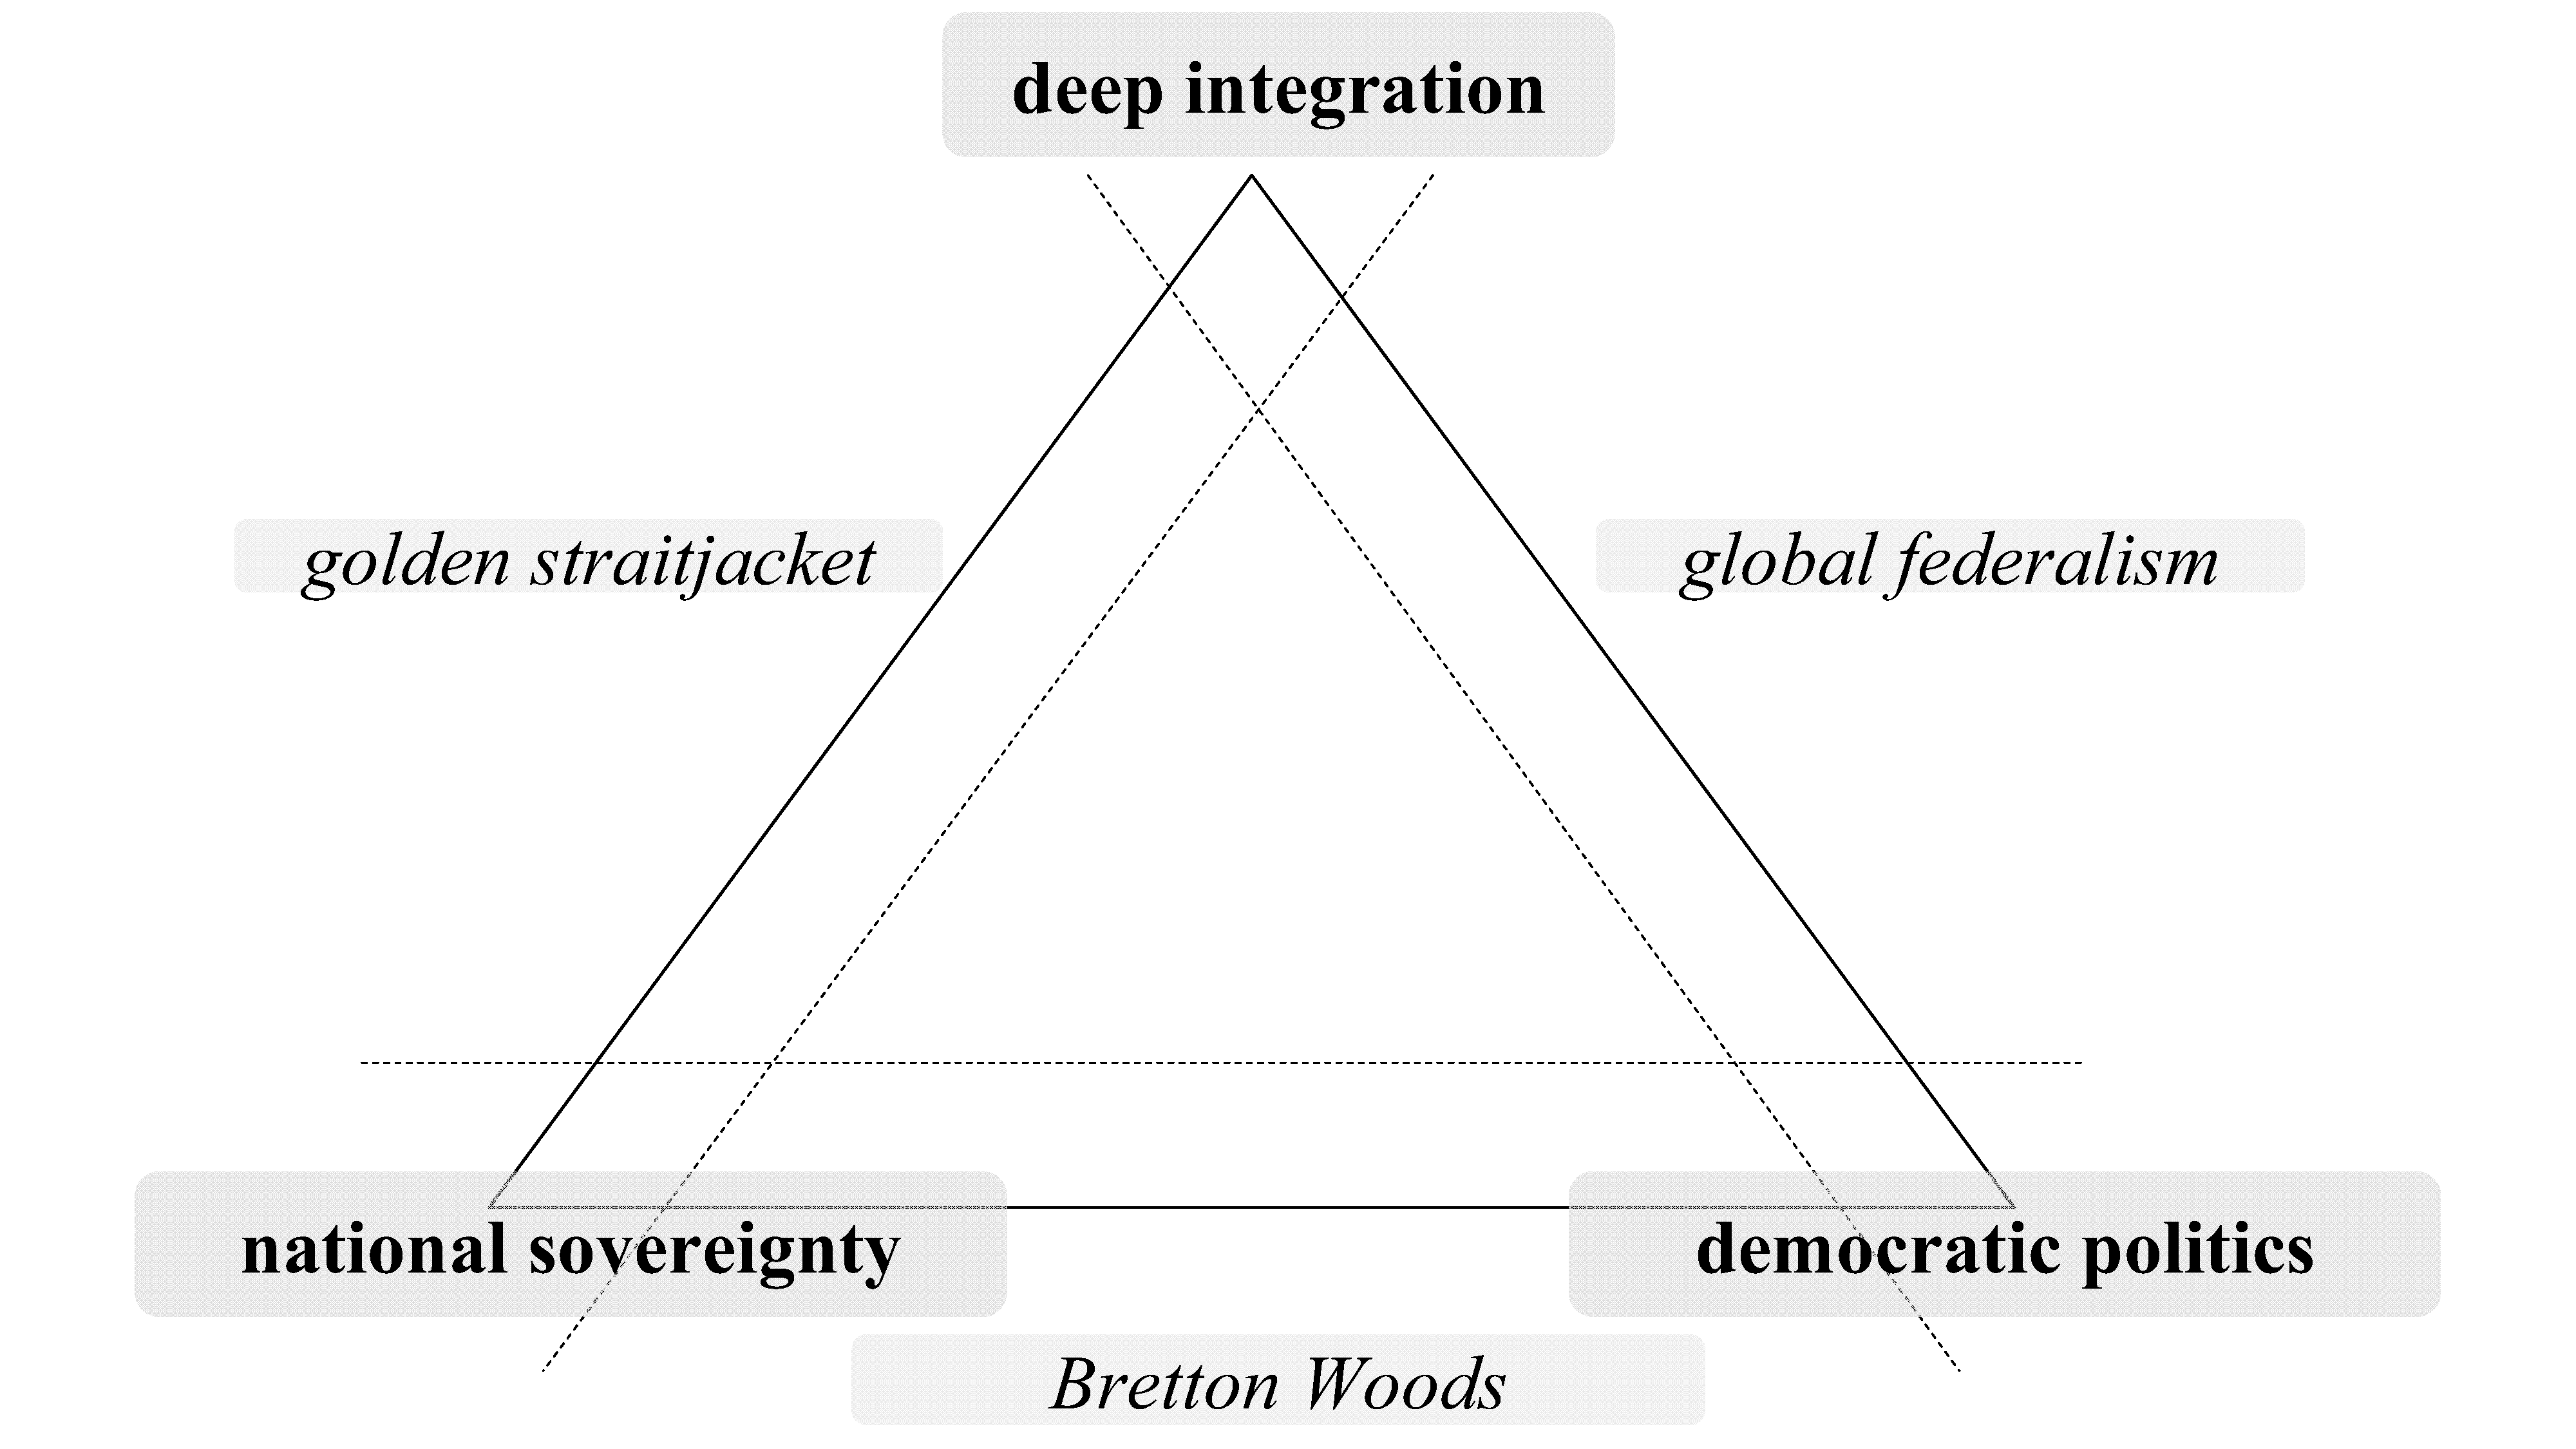
\includegraphics[width=1\linewidth]{ganssmann-macro-regimes}  
	\caption{Macroeconomic Regimes and Political Priorities}
	\label{fig:ganssmann-macro-regimes}
	\begin{flushleft}
		\scriptsize{\cite{Rodrik2002} as reproduced in \citeauthor{Ganssmann2010} (\citeyear{Ganssmann2010}: 348).}
	\end{flushleft}
\end{figure} 

\begin{figure}[htbp]
	\centering
	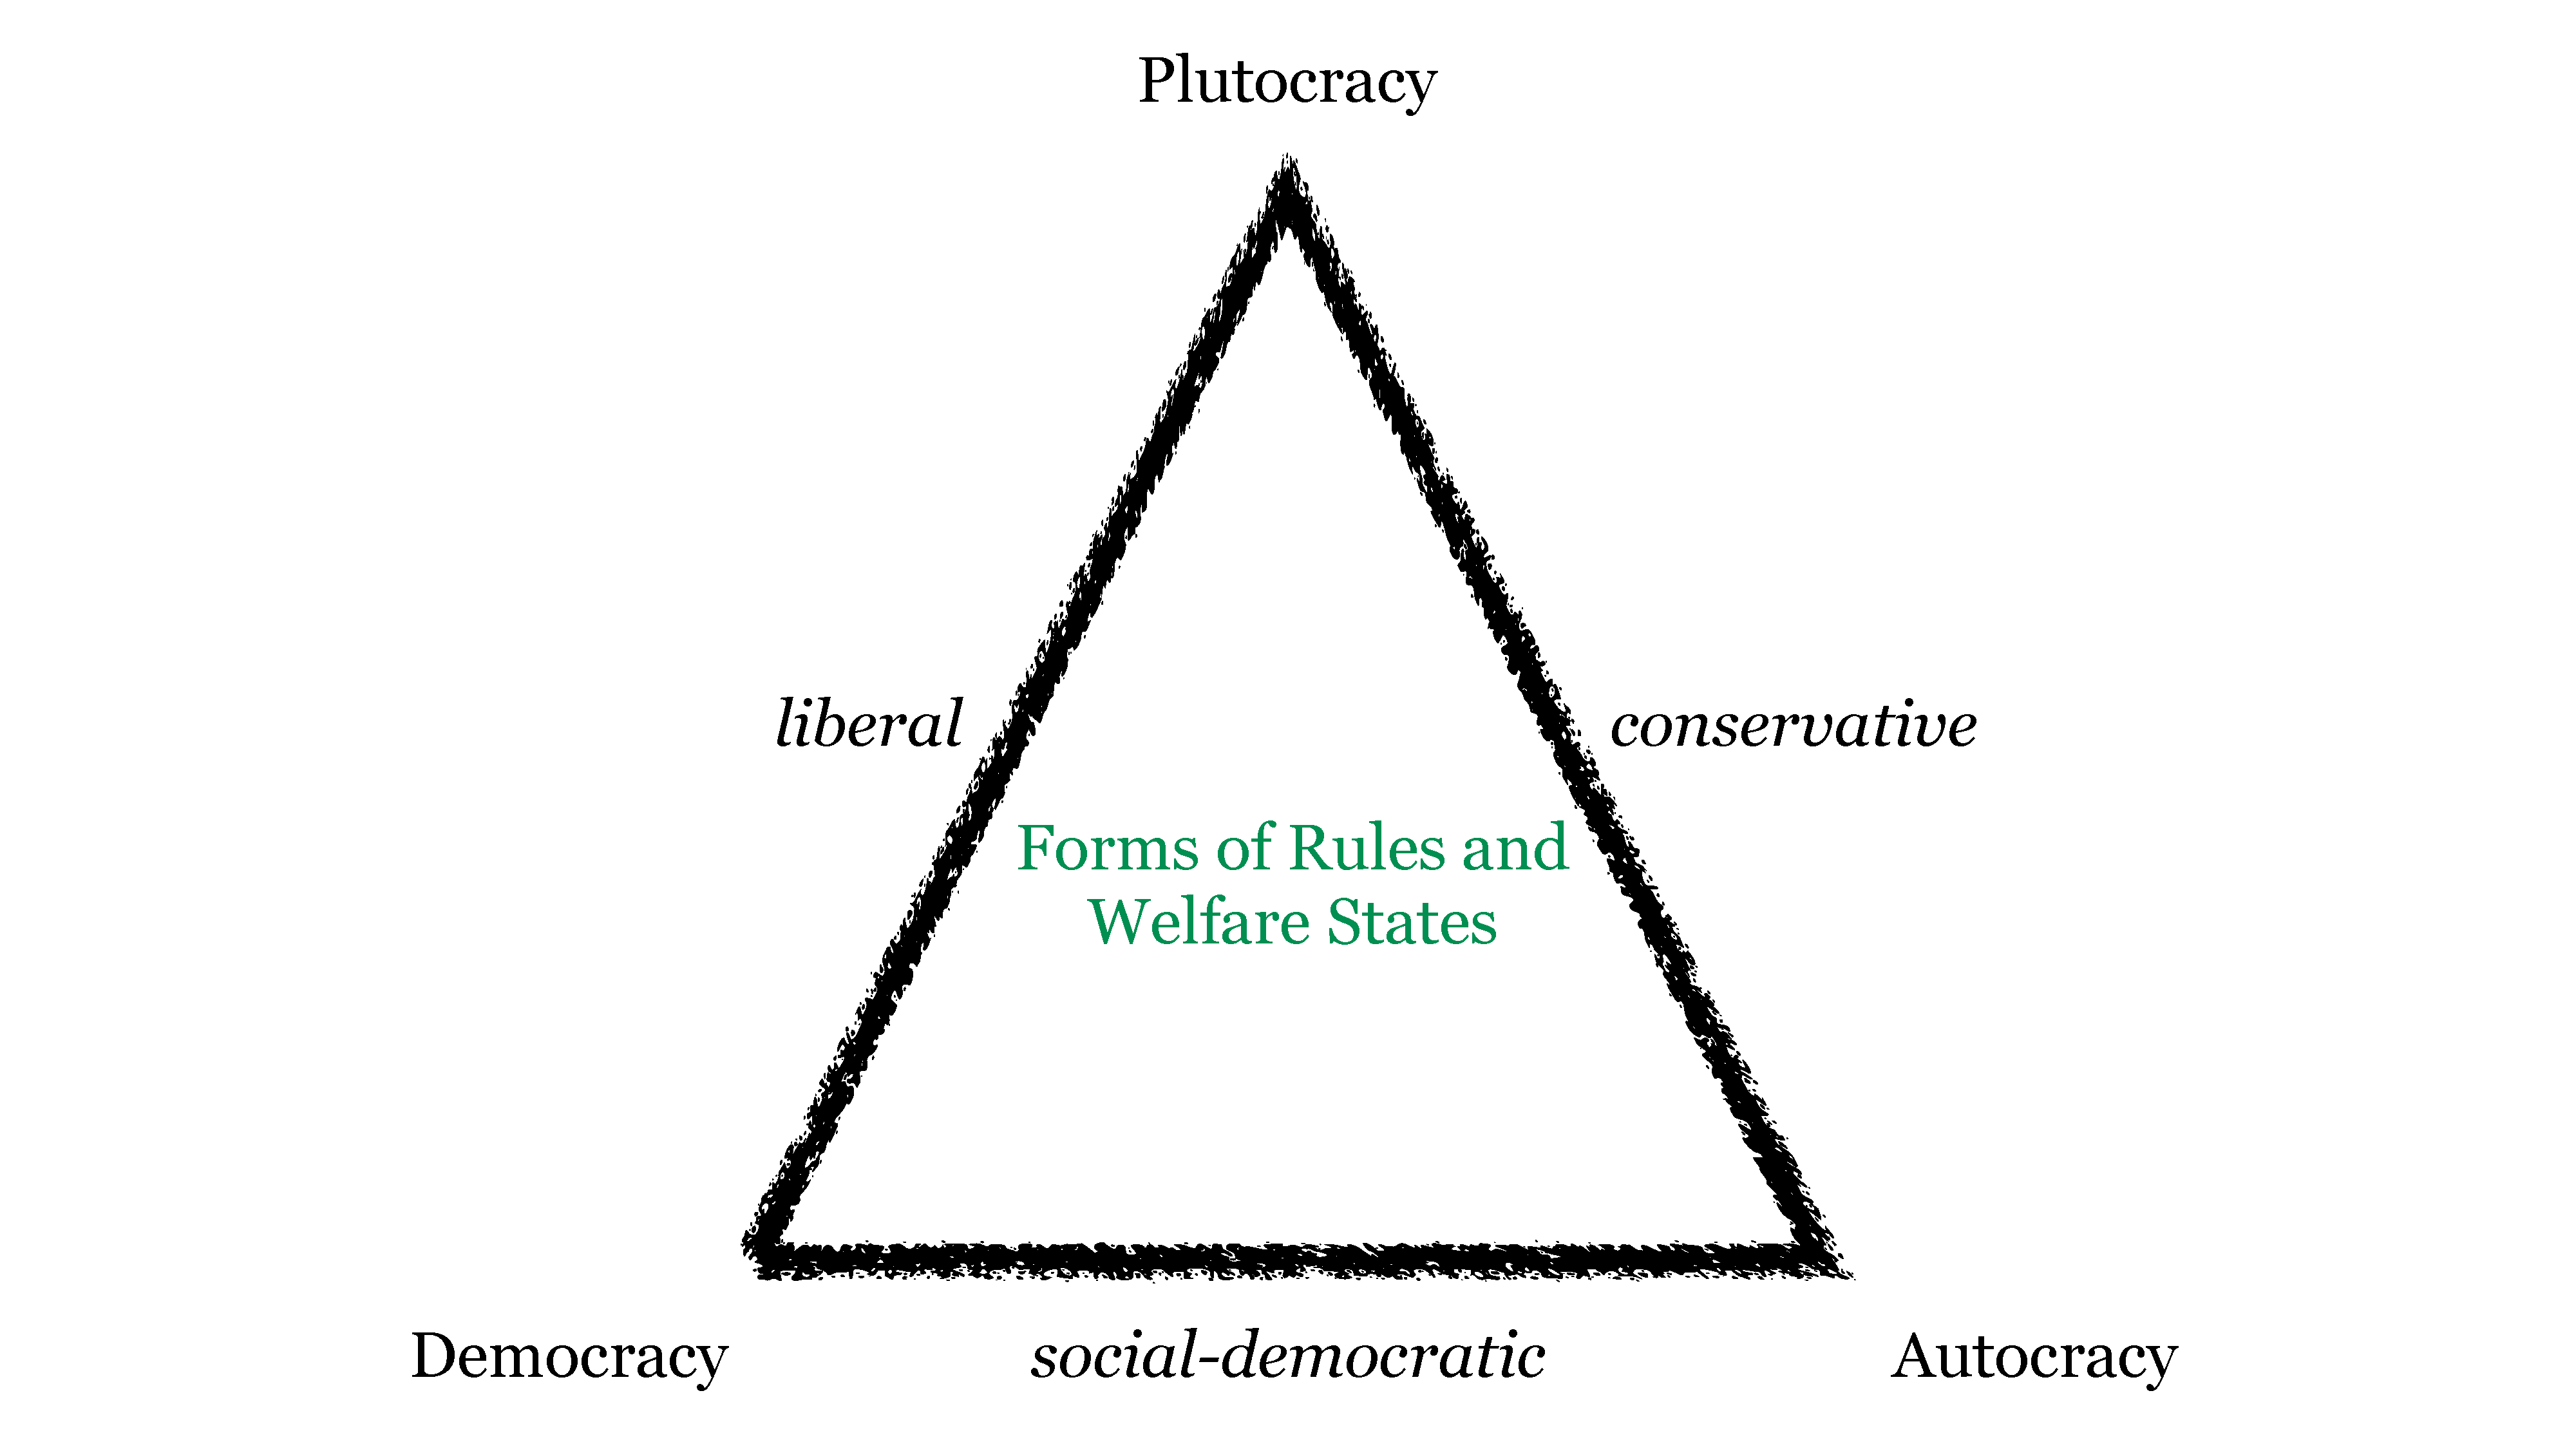
\includegraphics[width=1\linewidth]{ganssmann-rule-ws}  
	\caption{Forms of Rule and Welfare State Regimes}
	\label{fig:ganssmann-rule-ws}
	\begin{flushleft}
		\scriptsize{Reproduced from \citeauthor{Ganssmann2010} (\citeyear{Ganssmann2010}: 334).}
	\end{flushleft}
\end{figure} 

\begin{figure}[htbp]
	\centering
	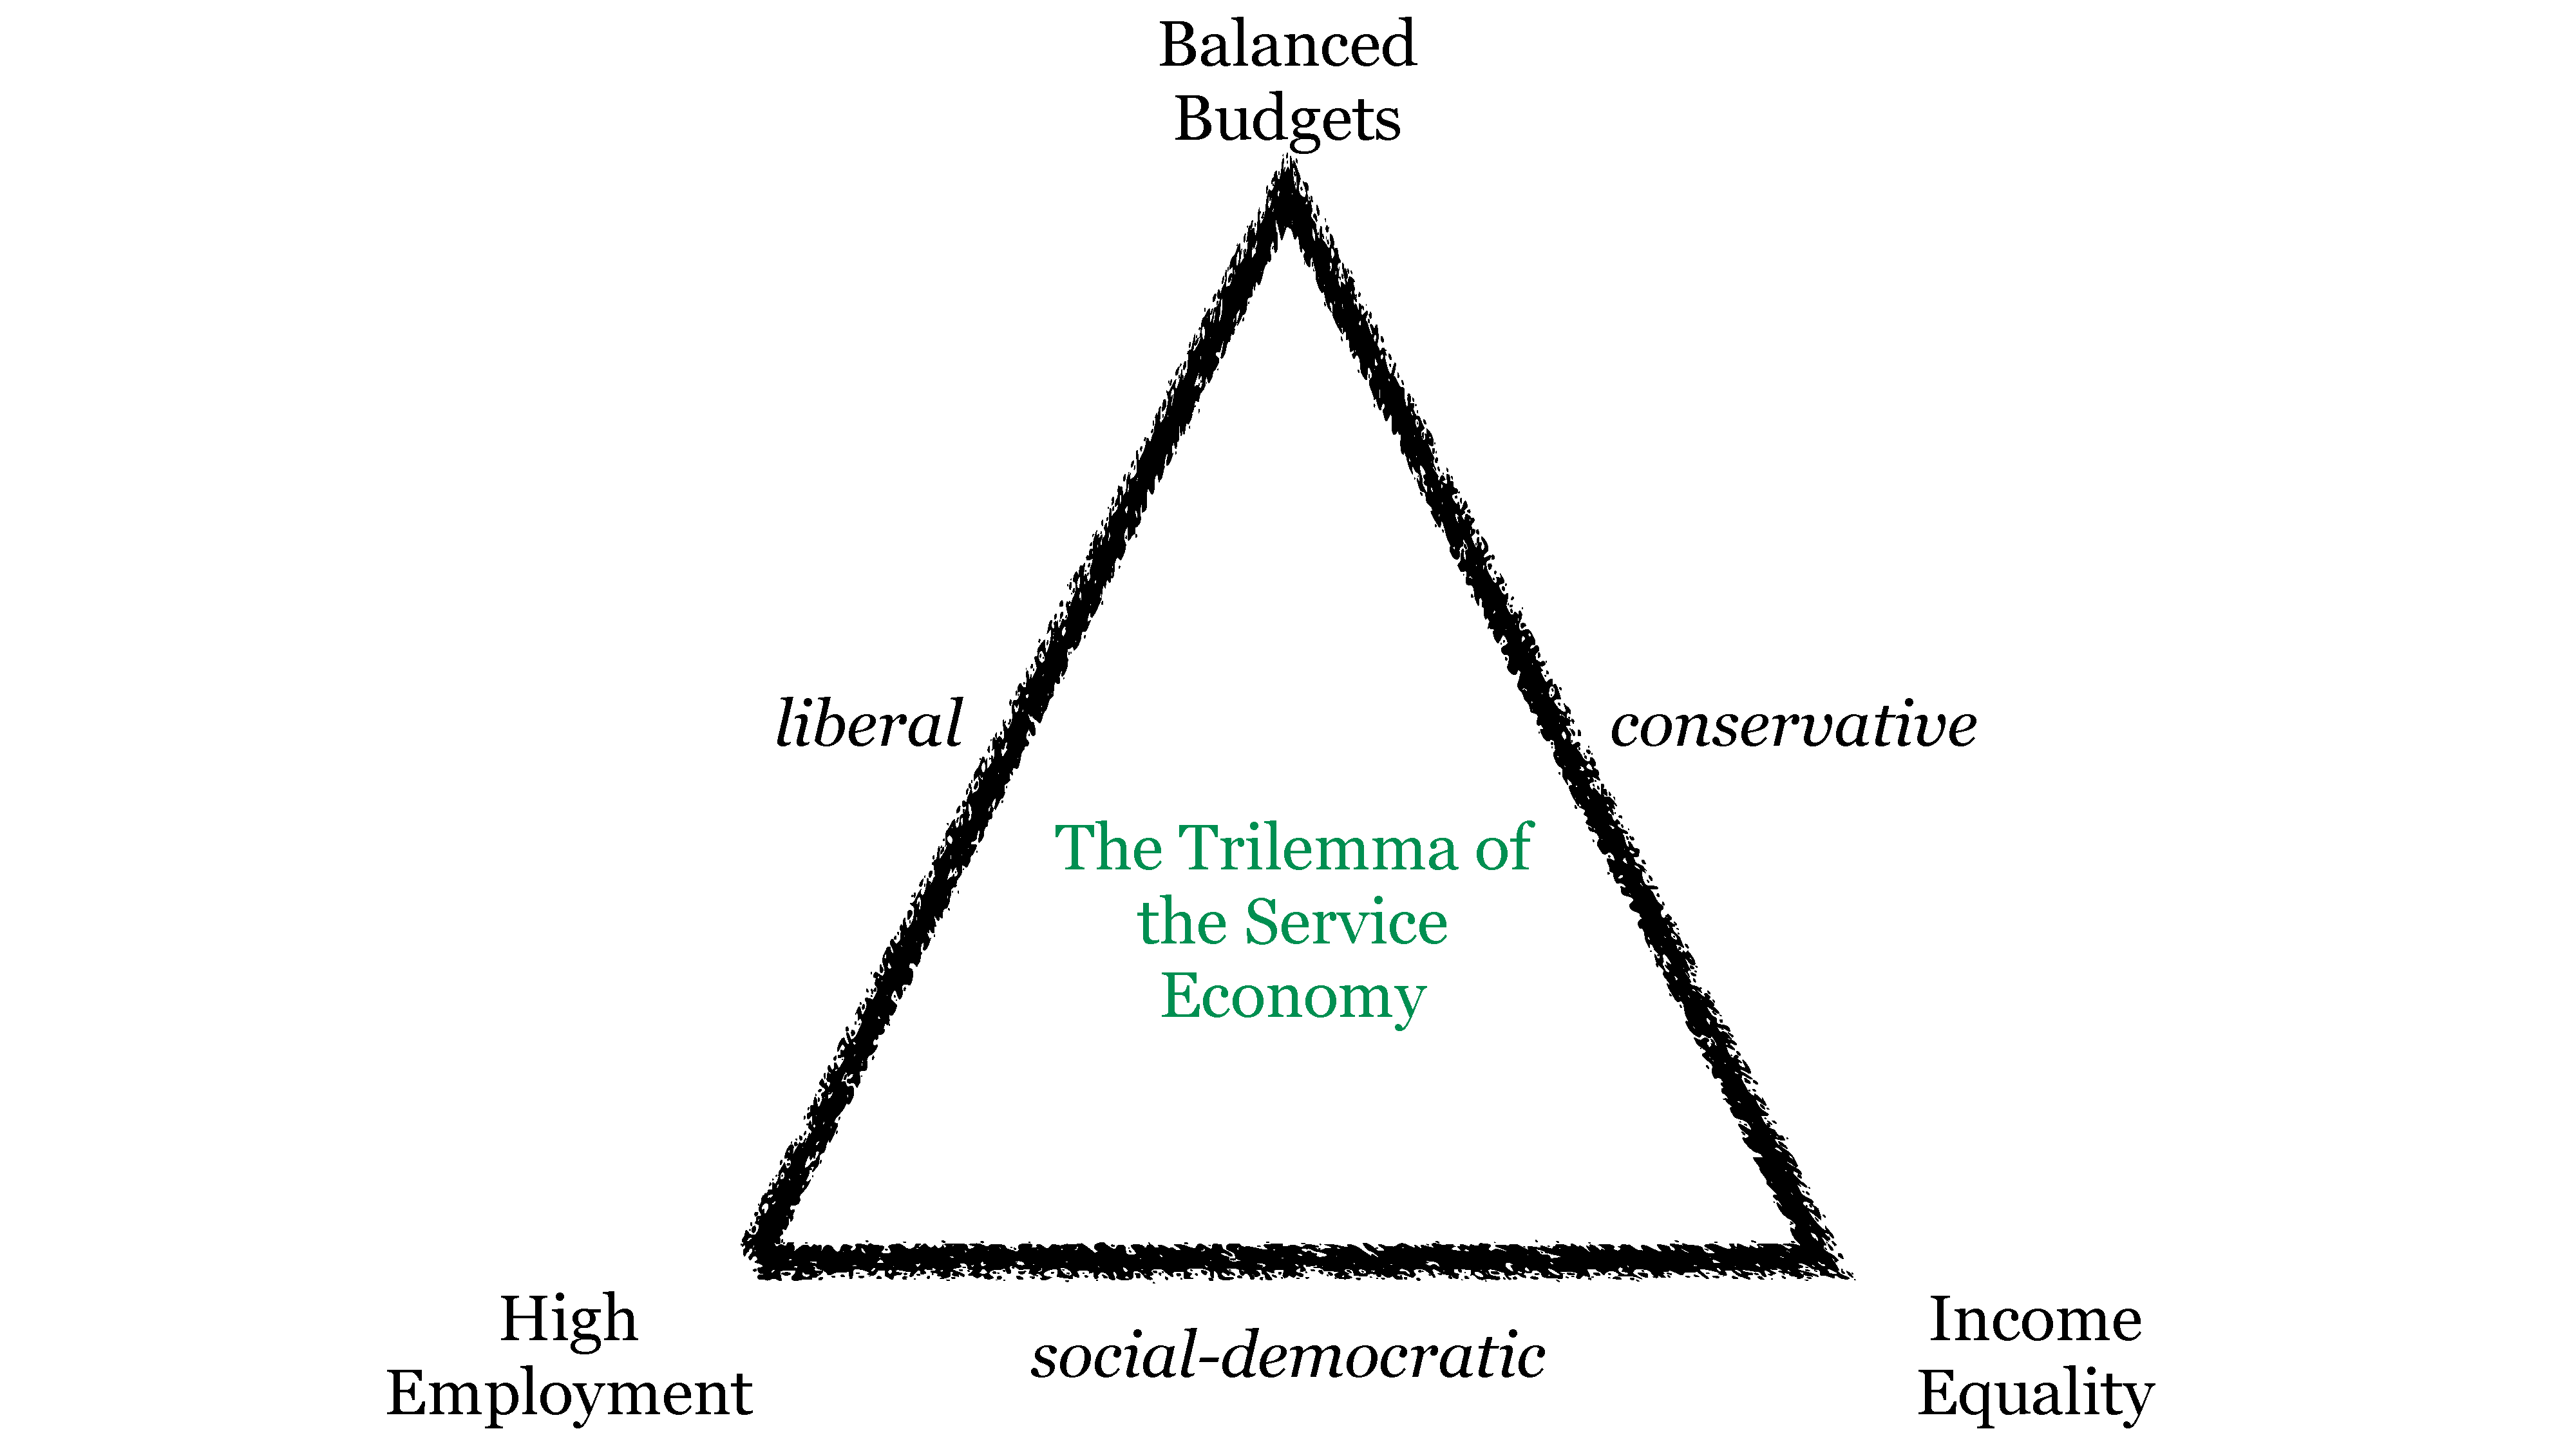
\includegraphics[width=1\linewidth]{ganssmann-trilemma-service-economy}  
	\caption{Trilemma of the Service Economy}
	\label{fig:ganssmann-trilemma-service-economy}
	\begin{flushleft}
		\scriptsize{Reproduced from \citeauthor{Ganssmann2010} (\citeyear{Ganssmann2010}: 341).}
	\end{flushleft}
\end{figure}

\begin{figure}[htbp]
	\centering
	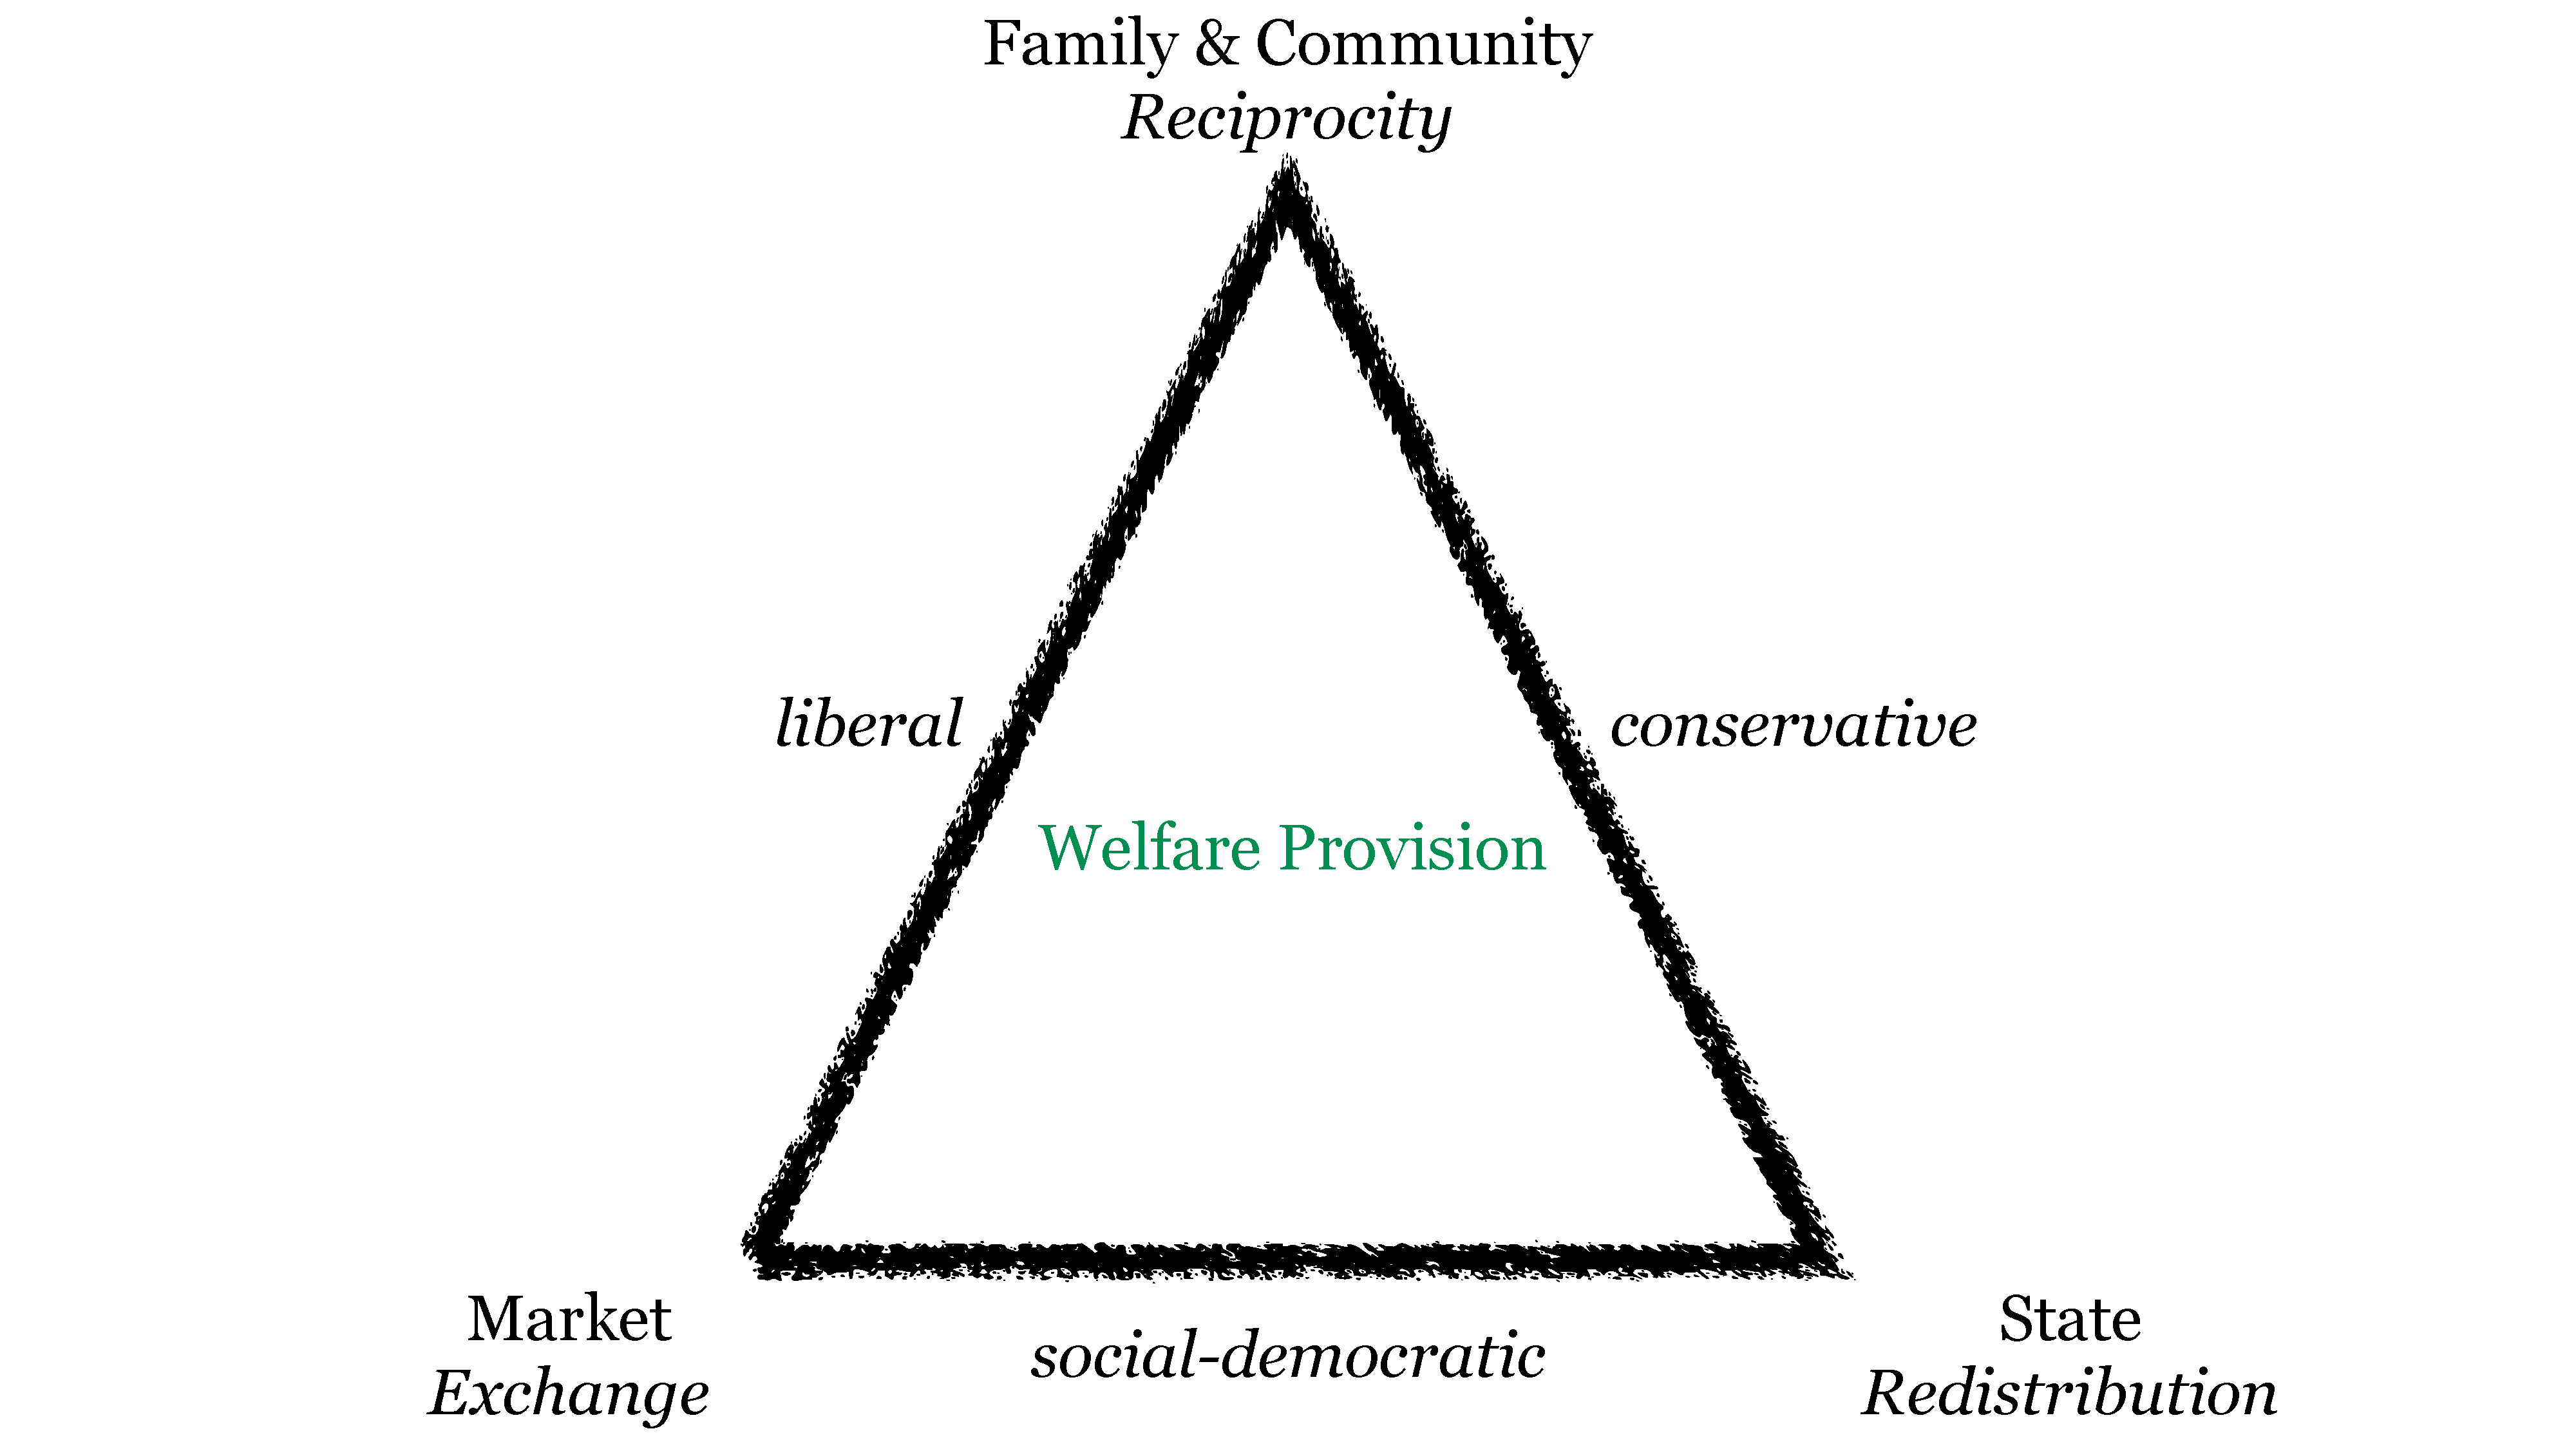
\includegraphics[width=1\linewidth]{ganssmann-welfare-provision}  
	\caption{Welfare Provision and Political Ideologies}
	\label{fig:ganssmann-welfare-provision}
	\begin{flushleft}
		\scriptsize{Reproduced from \citeauthor{Ganssmann2010} (\citeyear{Ganssmann2010}: 334).}
	\end{flushleft}
\end{figure}

%here used to be the ppf-tax-regimes, it's now in testing-hypotheticals

%ganssmann is absolutely crucial for the constrained alternatives.

%Four disclaimers apply:

%\subparagraph{Not Original.} The perspective I take here is hardly original. Many others have, in greater width \citep{Stiglitz2002} or depth \citep{Sinn2004}, with narrower \citep{Scharpf1997} or different foci \citep{Zurn-2000-aa} discussed the first-order shortcomings of regional integration in the \gls{EU}, and economic liberalization elsewhere \citep{Stiglitz2002}. I aim here to reasonably comprehensively review the works of others and to restate some fairly conventional economic concepts in order to build a first-order checklist of welfare state design. I then discuss in \autoref{sec:Literature} how much of the \hyperref[sec:Literature]{current literature lacks awareness} of alternative, possible and desirable welfare states and why that matters.

%\subparagraph{No Positive Test.} 

%why it matters, copied from the europe piece.
%add footnote

%McCaffery
	%our tax system is a disgrace, and has been so for decades. The way we tax is complicated, inefficient, and unfair. Yet whenever elected officials in Washington actually try to do something about tax, they tinker at best. At worst, they make the system even more annoying. We need fundamental, comprehensive tax reform, not ad hoc tinkering. Two, there is a widening gap between the rich and the not-rich in this country. It may surprise many readers to learn that there is a deep connection between these two facts. Tax as it is today is a cause of the wealth gap. Tax as it could be tomorrow would narrow it. That'sRead more at location 50   • Delete this highlight
	%Note: this is key. It's fucked up, but systematically so. Edit

%the below is from the europe piece, here comes th crisis of what happens when it doesn't work.

\subsection{Tax}

Taxation in the \gls{EU}, for the most part, remains an exclusive competence for \gls{MS}. Under the acquis, only indirect taxes (VAT) are harmonized --- at ineffective, minimal levels --- with very limited cooperation in other fields (for example, \citealt{EuropeanCommission2009}, \citealt{TaxCoordinationandTaxCompetitionintheEuropeanUnion-EvaluatingtheCodeofConductonBusinessTaxation2001}). Per its treaties, the \gls{EU} can harmonise only \emph{indirect}, always proportional taxes --- such as \gls{VAT} --- and only by \emph{unanimous} decision of the Council on proposals by the Commission (Article 113, Treaty of Lisbon, 2009 / Article 93, Treaty Establishing the European Economic Community, 1957). Union members do not even fully cooperate in collecting existing, national taxes: instead of full reporting of all incomes, some incomes (for example, dividends) and some countries (for example, Luxembourg) are exempted and instead levy a proportional, much lower withholding tax. It is, in short, no exaggeration to say that the \gls{EU} has no fiscal institutions or even coordination to speak of.

In the \gls{EU}, there is no match between the scope of economic activity --- the union-wide common market --- and the scope of taxation. 

With no union-level taxation, what does this mismatch do to 
\gls{MS}-level taxes? As the abstractions of the mixed economy suggest, tax competition results. For example, \cite{Genschel2009} find that tax competition is different and greater within the \gls{EU} than outside of it, and that it accelerates with time and enlargement. \gls{EU} tax competition is a \gls{PD}, where states (strictly) dominantly prefer low taxes over high taxes and (Nash) equilibriate in suboptimal, mutual low taxation (\autoref{tab:EU-Tax-PD}, p.~\pageref{tab:EU-Tax-PD}).

%!TEX root=../tax-democracy-held.tex

\begin{table}
	\caption{International Tax Competition, Stylized as a Prisoner's Dilemma}
	\label{tab:Tax-PD} %change label?
	\begin{center}
	\begin{tabular}{m{1cm}m{2,3cm}m{2,3cm}m{2,3cm}m{2,3cm}}
		& & \multicolumn{2}{c}{\emph{Home}} \\
		& &Low Tax& High Tax\\ 
		\cline{3-4}
		\multicolumn{1}{c}{\multirow{4}{*}{\emph{Rest of World}}} & \multirow{2}{2,3cm}{Low Tax} & 		\multicolumn{1}{|r|}{3} & \multicolumn{1}{r|}{0}\\ 
		\multicolumn{1}{c}{} & \multicolumn{1}{c}{}& \multicolumn{1}{|l|}{3} & \multicolumn{1}{l|}{10}\\ 
		\cline{3-4}
		\multicolumn{1}{c}{} & \multirow{2}{2,3cm}{High Tax} & \multicolumn{1}{|r|}{10} & \multicolumn{1}{r|}{7}\\ 
		\multicolumn{1}{c}{} & \multicolumn{1}{c}{}& \multicolumn{1}{|l|}{0} & \multicolumn{1}{l|}{7}\\ 
		\cline{3-4}
	\end{tabular}
	\end{center}
	\scriptsize{\emph{Home} and \emph{Rest of World} are the only two countries. They set their tax rates either high, or low. Capital and other mobile factors flow to whichever country has the lower tax rate. Payoffs are state revenues.}
\end{table}

If, and to the extent that such a race-to-the-bottom is at play in the \gls{EU}, it will affect both levels and schedules of national taxation.

\paragraph{Levels.} Straightforwardly, \gls{MS} will be strictly limited in the overall level of taxation they can sustain. Governments will no longer be free to set a level of taxation, or, equivalently, determine the command-exchange components of the mixed economy. In some cases, tax levels may even fall, as has been shown for \gls{CIT} rates \citep{Piatkowski2008}.

%re-read Piatkowski about this stuff.

\paragraph{Base.} Moreover, and more importantly, competition will also alter the base composition of taxation. To avoid large \glspl{DWL}, as they should, governments will turn to bases that are relatively price inelastic, that is, economic transactions that cannot be altered to escape taxation. \gls{EU} integration opens up a lot of new escape routes, especially for newly mobile capital, and, to a lesser extent, high-skilled labor: they can relocate their economic activity to wherever the tax burden will be lowest. This causes welfare-depressing distortions in the high-tax economy: rather than face a now voluntary tax, these pareto-optimizing exchanges will not be made at all, and instead happen elsewhere. For example, a rich entrepreneur otherwise willing to open a new factory in high income-tax Germany, may, faced with the new alternative of building the same facility in a low-tax location, forego his original plan. Germany unambiguously looses welfare, both because the investment is not made, and also because it does not even generate any fiscal revenue.

Faced with these dynamics, governments will, again rightly so, shift their taxation to bases that are less prone to \glspl{DWL}, or equivalently, bases that are relatively less mobile. Relatively less mobile bases in the \gls{EU} will be consumption and labor incomes, because consumers and workers cannot easily do their shopping and working in another country. 

Other --- partly dysfunctional --- taxes traditionally used to raise revenue for mixed economies will be rolled back or falter altogether. This applies especially to --- anyway defunct --- national \glspl{CIT} that large corporations can often evade easily, in part because nailing down the locale of any particular increment of income of a multinational firm will always be conceptually difficult. For example, the German holding of Deutsche Bank AG can easily reassign a particular income stream to a Luxembourg-based subsidiary, arguing that a crucial business process occurred there. Tax administrations will always, and necessarily, be unable to argue where any particular value was created (\citealt{Ganghof2006}, \citealt{Ganghof}, \citealt{Ganghof2007}: 5). Similarly, higher brackets of progressive \gls{PIT} will also cause large \glspl{DWL} or, more likely and wisely, disappear, as high-income individuals change residence or citizenship, offshore their income-generation to other countries, or at least shelter it in foreign corporations no longer affected by high, backstop \glspl{CIT}. For example, a rich German entrepreneur can establish a new holding in Ireland to buy up his German-based firm, and have it retain most if not all of the earnings, effectively escaping german income taxation. 

If and to the extent that Pigouvian taxes, or even fees fall on mobile bases, these will also either cause excessive market distortions, or, more likely, disappear. For example, a German steel producer may, (hypothetically!) faced with the German ecotax, relocate to Poland, avoiding the higher energy price, \emph{without}, as the Pigouvian tax intended, raising the price of steel. Overall energy intensity will remain the same, steel production will simply fall below equilibrium levels in Germany.

\paragraph{Schedule.} Crucially, by shifting the base, \gls{EU} \gls{MS} will also alter the schedule of their tax regimes. By relying more on taxing labor incomes, schedules will become more regressive: most large incomes in developed capitalist economies are not labor, but capital incomes. By relying more on (pre-paid) consumption and other indirect taxes, schedules will become regressive or --- at best --- proportional: even if rich people, just as others, eventually spend all their income, they will only pay the same percentage in \gls{VAT} or similar taxes. If union member governments wish to avoid, as they should, excessive \glspl{DWL} they will have to sacrifice progressivity in tax. The already impaired, but lone vestige of progression, the \gls{PIT} together with its ugly, but necessary backstop\footnote{
	Personal income taxes on capital necessitate a corollary taxation of corporate income. Without it, taxpayers could easily evade payment by incorporating capital it in a firm, withdrawing earnings only slowly.}, 
the \gls{CIT} will either disappear altogether, or, largely equivalent, depress their schedules and degenerate into effective labor income taxes, with, at best, some residual but proportional taxation of capital.

\subsection{Dysfunctions} \label{sec:defunct} What kind of an economic reality results from this open, but heterogeneous \gls{EU}, with unbounded trade, mis-configured currency union and rampant tax competition? It is, and must be, a deeply dysfunctional design, boxing the European household in unattractive policy dilemmas, wasting its communal resources, ever building new imbalances, harboring new crises, and, ultimately, fracture the social contract.

\subsubsection{Underfunding} \label{sec:public-squalor} Straightforwardly, the strictly limited revenues of \gls{EU} \gls{MS} confine them to structural underfunding, or at least, constrain the command-exchange \hyperref[sec:trade-offs]{trade-offs} that mixed economies are otherwise free to make (p.~\pageref{sec:trade-offs}). %add reference.
By subjecting taxes to competition, any increment in more command production and distribution must be bought at an increasing price in lost economic activity, or \gls{DWL}. 

In this scenario, governments rebalance their Haig-Simons identities --- as they always must --- by cutting public consumption or dissaving out of their wealth. This can take many, but entirely equivalent forms. For example, governments can save on public goods, such as road maintenance, or it can reduce transfer payments, such as welfare benefits. It can also dig into its savings, and take on new debt, or, let infrastructure fall into disrepair.

Here, too, government is faced with unattractive choices: to either cut public spending to suboptimal levels, to go into debt or to otherwise dissave.

%need evidence

\subsubsection{Unemployment}
The neoliberal agenda promised that if states cut their spending, at least their economies would greater economic growth. Under a dysfunctional mixed economy, that is not necessarily so. In the \gls{EU}, mixed economies cannot have the cake and eat it, they cannot even do one of the two. Instead, its welfare states are faced with a twin crisis that is mutually reinforcing: one of structural unemployment, and one of structural underfunding, as illustrated in \autoref{fig:twin-crisis} (p.~\pageref{fig:twin-crisis}). 

Structural underfunding, aside from causing \hyperref[sec:public-squalor]{public squalor} (p.~\pageref{sec:public-squalor}), in the long run may also diminish the kind of public and common goods that drive future economic growth, such as basic research or infrastructure, and especially, education. Over the long haul, structurally underfunded states will ill-equip workers for a global marketplace, and leave them with comparatively poor labor productivities.

In addition, structurally underfunded governments are increasingly unable to transfer  low- and middle-income workers, or, at least, exempt them from taxation. In particular, the greater tax burden on immobile labor, and the constrained progressivity of tax under competition will make it even harder for workers to make ends meet at any given market income. They have to pay more --- not less --- to the state, or, misleadingly named ``social insurance'' and keep even less for their personal consumption.

As a result, at least some workers will be relatively unproductive and face high taxes on their already low or middle market incomes. If and to the extent that \gls{EU} welfare states maintain some minimum socially acceptable living standard, either through a minimum wage, or, equivalently, welfare transfers, these low and some middle income earners will find it increasingly difficult to earn enough on the market to meet this standard. Any --- already diminished --- income will be further depressed by a tax wedge driven between the gross and net disposable incomes. Both in a minimum wage, and a welfare transfer regime, those workers with productivities too low to make the minimum income on the market will exit the market, and collect welfare instead --- not out of laziness, but out of necessity. 

The ensuing structural unemployment, in turn, reinforces the structural underfunding of the mixed economy government. First, it creates greater needs for transfers, putting further strain on public transfers. Secondly, it also depresses growth, and in the long run, diverges the economy from its long-term growth path, as segments of the labor force lie needlessly idle.

%here used to be \ref{fig:dual-crisis}, now only in 3-crises

Alternatively, of course, governments can lower effective price floors by cutting welfare benefits, minimum wages or by raising work requirements. By lowering minimally acceptable social standards --- frequently euphemised as ``structural realignments'' or ``labor market flexibility'' --- states will have to abandon central welfare tenets and create and accept, once again, widespread working poverty. %add some butterwegge results here.
That is, \gls{EU} welfare states can brake the vicious cycle of underfunding and unemployment if they cease to be welfare states, a configuration that \cite{Streeck2010c} has aptly called a ``permanent austerity regime''. %visualize this already as an unattractive choice?

Governments of dysfunctional mixed economies, here, as always, are faced only with equally unattractive options: to either save social standards at the price of structural unemployment and depressed growth, or to abandon them and risk widespread working poverty.

This dual crises, and the uneasy choices it forces, will only be exacerbated in a modern and open economy. Modern economies already produce highly unequal returns, as winners take all and, equivalently, Baumols cost disease looms. A modern economy will, by its very structure tend to produce people whose productivities are much lower than the overall productivity of their host countries. %add hyperref.  
Trade, migration and capital mobility add even more pressure. As countries specialize even more according to their factor endowments (think: Romanian Nokia, German Management Consulting), remaining, relatively scarce factors (think: unskilled laborer in Germany) may find their market wages fall even further below the respective socially acceptable minimum income. Especially rich states may then be forced to redistribute income to these individuals, but find themselves unable to raise the necessary revenues (progressively) without further reducing their competitiveness. 

%need evidence

\subsubsection{Inequality} Lacking any union-level fiscal institutions and marred by tax competition between the \gls{MS}, the \gls{EU} mixed economy lacks effective tools to redistribute market outcomes. Both \emph{within} and/or \emph{between} member states, rampant inequality will remain unchecked, or even further widen.

At home, the mixed economy has lost its ability to dampen (possibly accelerating) winner-take-all dynamics, and to compensate the loosers from trade and economic transformation (for example, \citealt{Beckfield2006}\footnote{
	\citeauthor{Beckfield2006} finds for the \gls{EU}-12 that nearly half of the rise in within-country inequality between 1973 and 1997 can be explained by regional integration for example, (\citeyear{Beckfield2006}: 979).}): 
inequality almost everywhere in the \gls{EU}, has been widening, at least in part due to regional integration (for example, \citealt{DaudUngl2008}: 265). The great U-turn back towards more inequality, in Europe as elsewhere in the \gls{OECD} is well under way \citep{AldersonNielsen-2002-aa}. As tax competition both erodes the base and depresses the progressivity of taxation, market allocations, increasingly, are final. Moreover, structural underfunding and associated public squalor will also hit hardest the lower and middle income earners, further widening the divide in living standards. Rich people can afford to exit from public provision, for example by paying doctors out of pocket, by sending their children to private schools or even walling their gardens and gating their communities. Lower and middle income earners have no such exit option, but are stuck with decrepit public provision.
%need evidence

Between \gls{MS}, too, inequality will remain unchecked, as member and union level governments have no instruments to alter distributive dynamics of trade, that may --- or may not --- lead to fast convergence of productivities, and related, living standards. What is worse, the poorer mixed economies are especially constrained: at low productivities, they can least afford to burden mobile capital, and other mobile, high-earning factors, such as professionals with any, let alone progressive taxation. With open borders, but without coordinated tax or union-level transfers, these poorer \gls{MS} currently can only take the hard, unmitigated route to economic convergence: they tax mostly (low-productivity) labor, proportionally if not regressively, and at low overall public spending levels (for example, \cite{DaudUngl2008}: 267). By contrast, in the higher-productivity, rich \gls{MS}, corporatist arrangements, strong trade unions and substantial, if increasingly dysfunctional welfare regimes can still eek out pockets with sometimes generous welfare provision: in always capital-intensive, often high-value add and sometimes oligopolistic --- not commodity ---production, these economies can, at least in some sectors, afford welfare. For example, a Bavarian specialist engine builder with high capital and relatively low labor inputs and maybe a handful competitors on the world market,  may, faced with strong unions, accept above-equilibrium, possibly efficiency wages. Not so in Romanian manufacturing: Producing low-margin commodities, with little capital but hundreds of competitors and easy access, firms have to compete tooth-and-nail on labor costs. And so, \gls{MS} may not only fail to converge as quickly, or as closely as they could, or hoped to, but the very \emph{conditions} for economic development will diverge widely. The rich, high-productivity \gls{MS} can still, if inefficiently and incompletely, dampen and distribute the pain of whichever economic shock hits or transformation sets in. In the poor, low-productivity East and South, it will be bare-bones laiss\'{e}z-faire capitalisms\footnote{
	\citeauthor{Galbraith2002a} (\citeyear{Galbraith2002a}: 25) precisely describes an analogous, worldwide dynamic:
	\begin{quote}
		``In sum, it is not increasing trade \emph{as such} that we should fear. Nor is technolocy the culprit. To focus on `globalization' as such misstates the issue. The problem is a process of integration carried out since at least 1980 under circumstances of unsustainable finance, in which wealth has flowed upwards from the poor countries to the rich, and mainly to the upper financial strata of the richest countries. In the course of these events, progress toward tolerable levels of inequality and sustainable development virtually stopped. Neocolonial patterns of center-periphery dependence, and of debt peonage, were reestablished, but without the slightest assumption of responsibility by the rich countries for the fate of the poor. It has been, it would appear, a perfect crime. And while statistical forensics can play a small role in pointing this out, no mechanism to reverse the policy exists, still less any that might repair the damage. The developed countries have abandoned the pretense of attempting to foster development in the world at large, preferring to substitute the rhetoric of ungoverned markets for the hard work of stabilizing regulation. The prognosis is grim: a descent into apathy, despair, disease, ecological disaster, and wars of separatism and survival in many of the poorest parts of the world. Unless, of course, the wise spirits of Kuznets and Keynes can be summoned back to life, to deal more constructively with the appalling disorder of the past twenty years.''
	\end{quote}}.

In the \gls{EU}, Kuznet's and Keynes' grand hopes, that welfare would --- and should --- always follow growth, are dashed (as cited in \citealt{Galbraith2002a}: 22). If they have any choice at all, it is a very unattractive one for the governments of the union: they can either stay in the common market and reap the gains from trade and abandon all or some welfare, \emph{or} they can exit the union, stall economic integration, save their welfare regimes and retreat to autarky and recession.

\subsubsection{Imbalances and Crises} \label{sec:imbalances}

\begin{verse} 
	\href{http://www.npr.org/blogs/money/2012/03/01/147720368/50-ways-to-leave-your-lender}{50 Ways to Leave Your Lender}
	
	The problem is all inside your head, she said to me,\\
	You can't pay back 200 percent of GDP,\\
	You have to negotiate, if you want your country free,\\
	There must be 50 ways to leave your lender.

	You really don't want the IMF to intrude,\\
	Furthermore, they'll force austerity for the interest that's accrued,\\
	Imagine your middle class, subsisting on cat food,\\
	There must be 50 ways to leave your lender.\\
	Fifty ways to leave your lender.

	You just stretch out the loan, Joan,\\
	Cut the creditors' hair, Claire,\\
	Or boost GDP, Lee,\\
	Just listen to me.

	Print more money, honey.\\
	No need to pay back, Jack!\\
	Structure a default, Walt.\\
	And get yourself free.\\
	--- Planet Money / National Public Radio, 2012
\end{verse}

Democratic governments, firms and households alike will be under great strain from the underfunding, unemployment and inequality that a dysfunctional mixed economy creates. %add hrefs.
They may take on any possibility to temporarily relief the pressure they are under, even if it will not solve, or even exacerbate the situation in the long run: here, too, humans and the institutions they man, suffer from time inconsistency.

In modern financial capitalism and complex societies, there are some powerful painkillers to numb the effects of a dysfunctional mixed economies. As painkillers go, they treat the symptoms, not the disease, and have serious side effects. And so it is with the macroeconomic temptations in the \gls{EU}: as powerful drugs, they seemingly let economies transcend their material means, spread euphoria and frenzy. Only their cure is, ultimately, delusional, their treatment addictive. While under the charm of such chimerical boom and prosperity, economies keep building pressures and imbalances, that, one day, will unload in financial shocks and systemic crises, that, if sufficiently large, can disturb or bring down entire markets. After this kind of ecstasy always comes a day of reckoning, with a catastrophic hangover.

Just when an economy is in such drug-enduced delusion, and living beyond its long-term growth path is, as always in uncertain markets, hard to tell. National balance of payments accounts provide as in \autoref{fig:BoP} (p.~\pageref{fig:BoP}) an intuitive, if rough-and-dirty first indication. Between economies, too, an identity akin to Haig-Simons and the conservation of matter, holds: for any good or service that leaves the country, there must ultimately be imports of equal value, or, a change in ownership of foreign assets, that is, the promise of \emph{future} imports of goods and services. Conversely, any import must be matched by exports of equal value or it will be offset in \emph{foreign} ownership of domestic assets, that is, claims against future domestic production. As all the most important economic abstractions, this one is simple: balance of payments accounts are double-entry bookkeeping, only at the economy level.  

The components of balance of payments accounts, as the Haig-Simons identity, break down over households, firms and governments. For example, in a fictions German account, households can import olive, or firms can import particle filters as semi-manufactured inputs, or governments can import commuter trains for public transportation (\autoref{fig:BoP}, p.~\pageref{fig:BoP}). In these accounts too, positions of one owner are offset by positions of other owners in the same economy. For example, German household exports of home-made cuckoo clocks can be offset by said firm imports of particle filters in a roundabout way, when clockmakers buy French-particle-equipped German cars, or following some other chain of exchanges. Positions  also offset across the equality sign. For example, German household imports of olive oil may be offset by government issues of German bonds to Greek oil producers, with the government channeling the revenue to oil-consuming welfare recipients, or through a myriad of other transfers.

\begin{figure}[htbp]
	\begin{center}
	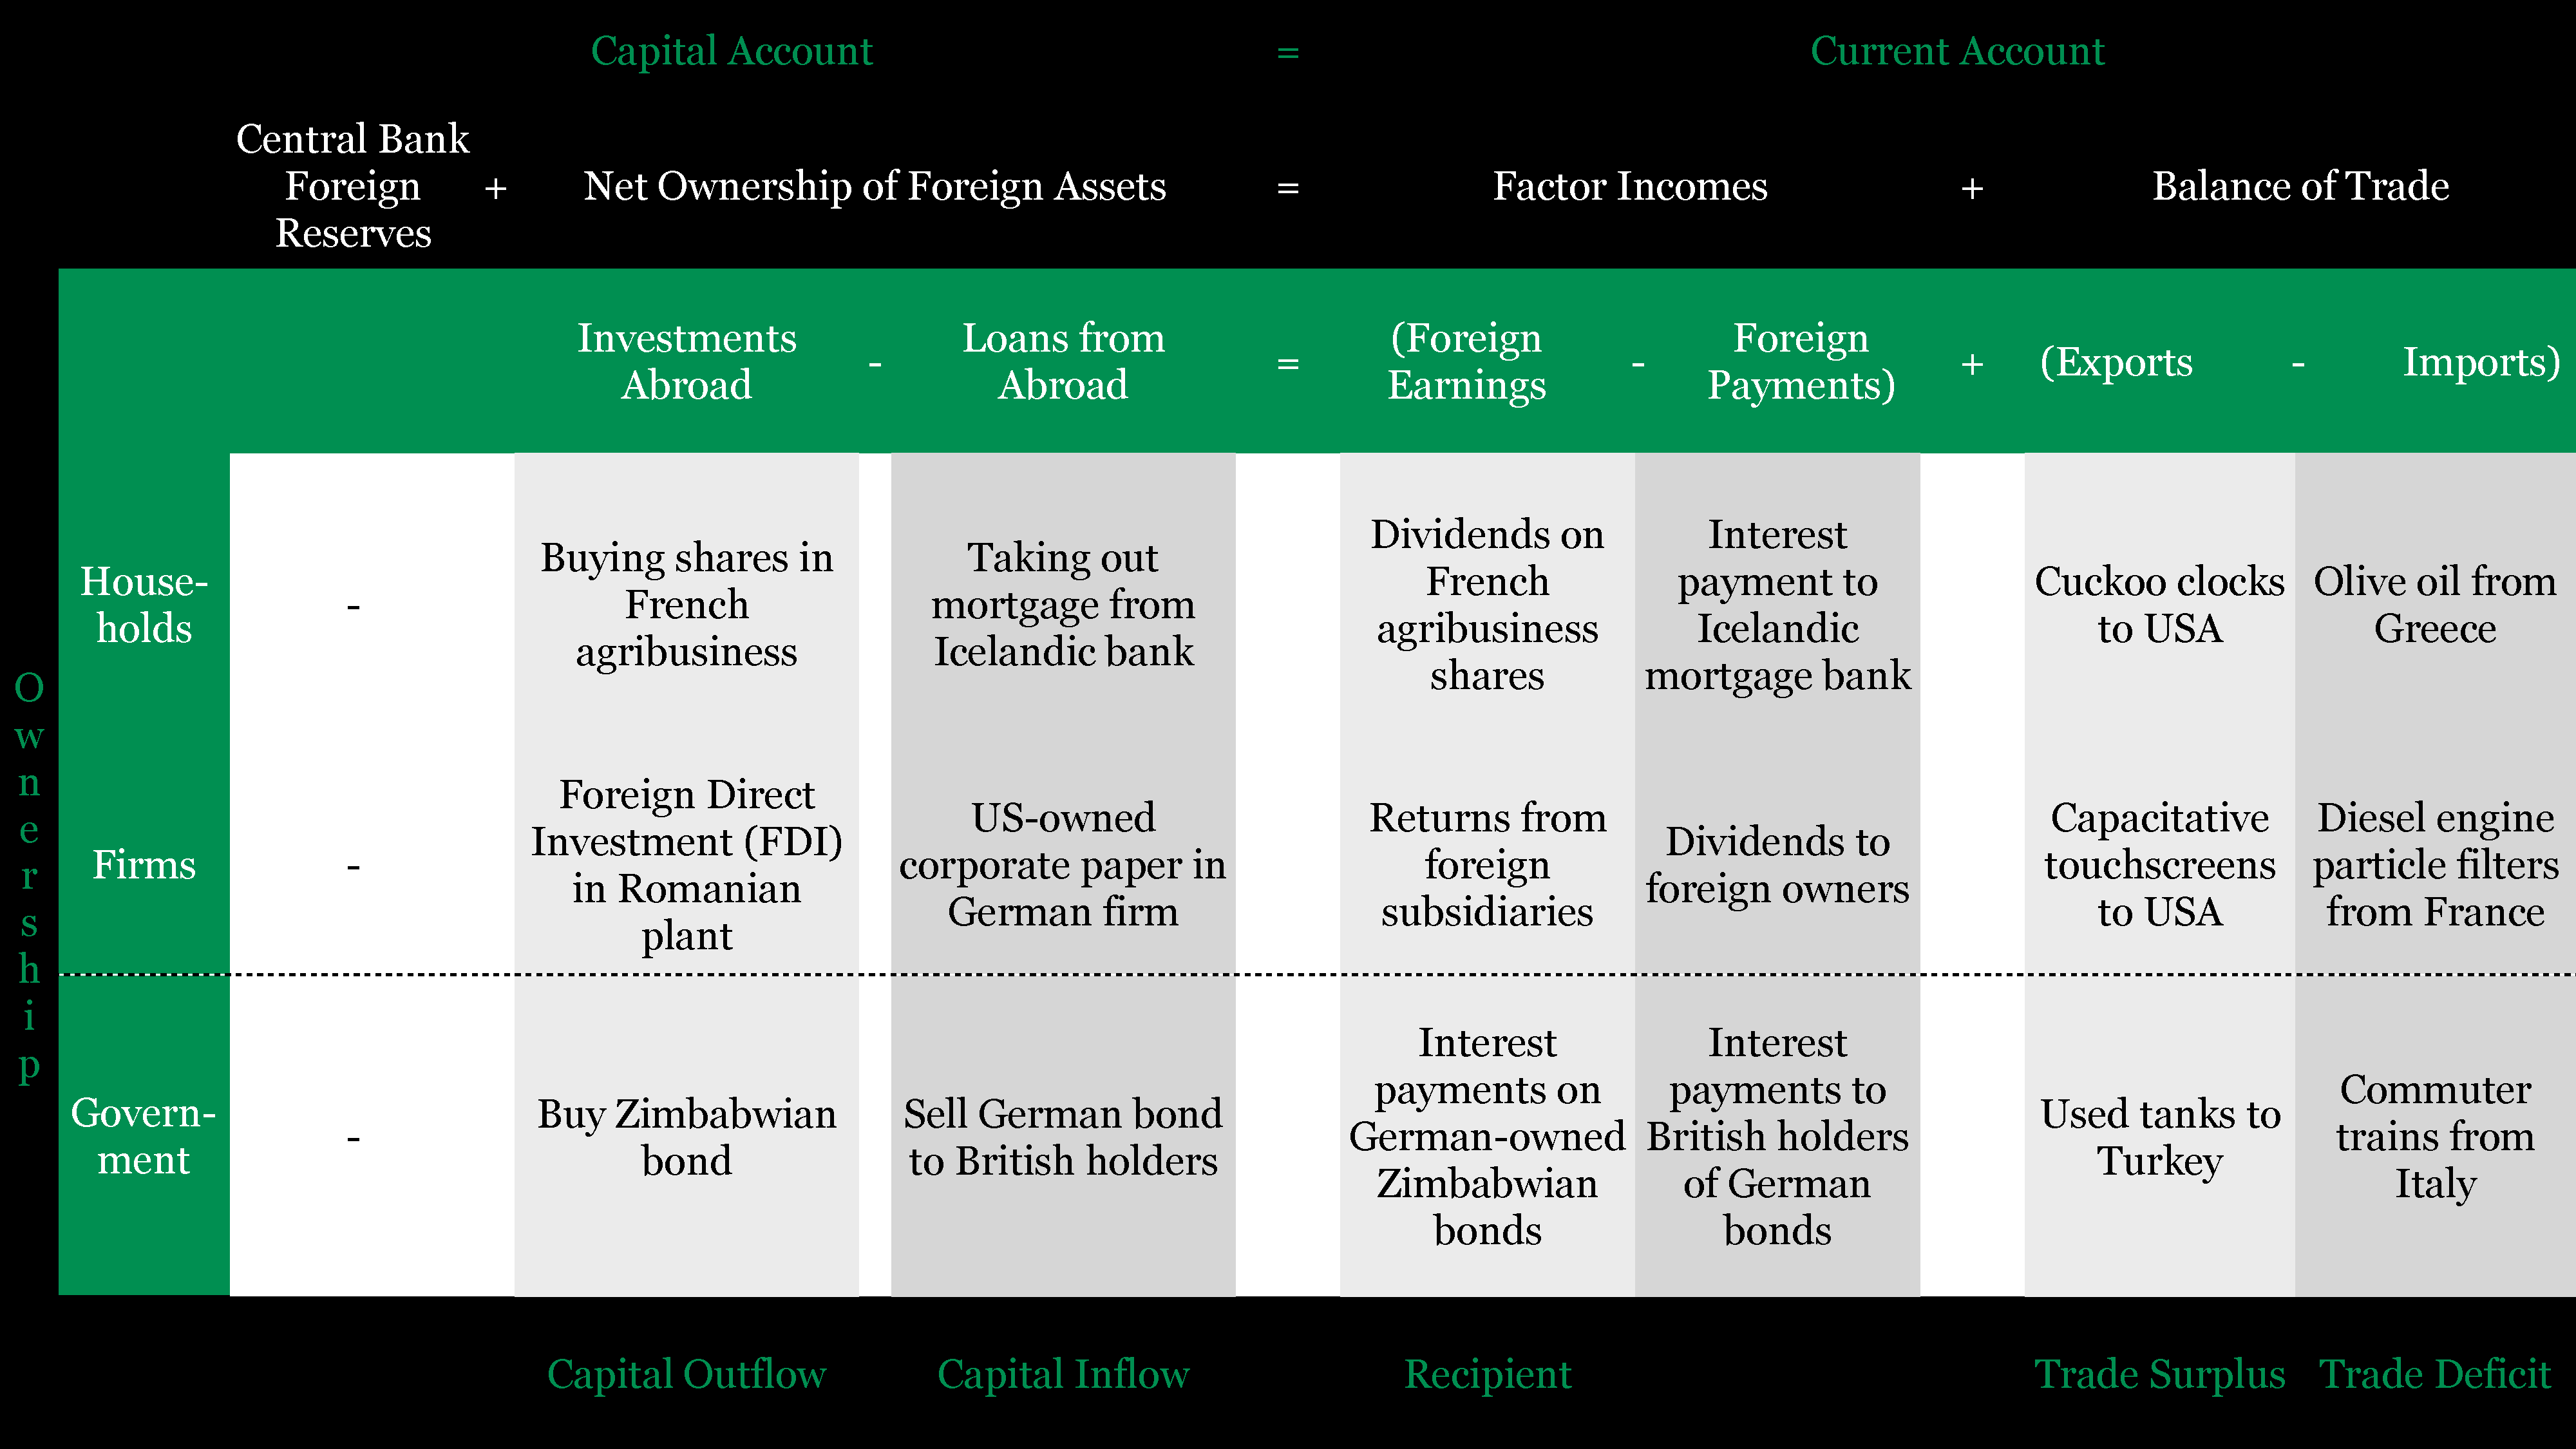
\includegraphics[width=1\textwidth]{balance-of-payments}  
	\caption{A (German) Balance of Payment Account with Examples}
	\label{fig:balance-of-payments}
	\end{center}
\end{figure}

Balance of Payment accounts are easily misunderstood or oversold, for a four reasons:
\begin{enumerate}
	\item Trade deficits and surpluses between any pair of countries are frequently reported, but meaningless and entirely unproblematic, just as shoppers need not worry about a trade deficit with the local supermarket. Trade deficits --- as consumer debt --- are potentially worrying only if they are \emph{net} of all exchanges with all trading partners.
	\item Conversely, balance of payments accounts do not apply  only between countries, as is easily assumed, but is, in fact a meaningful and true identity between any group of market participants and the rest of their trading partners, all the way down from nations to households. For example, a trade deficit may also arise between laggard regions, impoverished demographics or even generations, and the rest of an economy, with much the same possible problems.
	\item In the short term, even such trade deficits may not be problematic, but, in fact, help to stabilize economies from exogenous shocks. %reference OCA argument
	\item Even in the medium and long run, persistent trade deficits may be ok if and to the extent that the resultant capital inflows can reasonably be expected to currently, or in the future, earn whichever factor income was promised. For example, emerging economies may well experience persistent trade deficits for some time, while machinery is imported to equip the workforce, if and to the extent that the resulting, now capital-deepened production pays off as expected.
\end{enumerate}

Still, balance of payments accounts are an immensely enlightening abstraction, without which trading mixed economies cannot be well understood:
\begin{enumerate}
	\item Trade deficits are not a sufficient, but still a necessary condition for building macroeconomic imbalances. Not every trade deficit will betray an economy living beyond its means, but every economy artificially held above its long-term growth path by said financial drugs \emph{will} leave a grave trade deficit in its wake.
	\item The balance of payments identity shows, as Keynes  argued forcefully, if somewhat ineffectively at the Bretton-Woods conference in 1944, that these macroeconomic imbalances know no \emph{one} culprit. The loaded language notwithstanding, both deficit \emph{and} surplus economies are, equally, at fault. One parties excessive imports are another parties dumping exports. To get to equilibrium, where imports equal exports, either of the two parties, or both, must change its prices. To pride oneself, as German leaders frequently do, in being an export champion --- but not an import champion --- is but a mindless return to the folly of beggar-thy-neighbor, and, before that, mercantilism.
	\item Financial flows always track flows of tangible goods and services, as well as vice versa.
	\item It does not much matter \emph{who} --- households, firms or government --- in an economy creates the trade deficit. Only the deficit net of all economic actors in a given region matters. 
\end{enumerate}

How, then, do we know the acceptable trade deficits, from the unsustainable ones? We look at the offsetting changes in the capital account, and check whether these are intertemporally efficient, or whether they were enabled by failed markets. In the \gls{EU}, as in any other mixed economy, we must beware of these smoke and mirrors, that only forestall and worsen the inevitable day of reckoning: credit bubbles, asset bubbles, inflationary pressure, and nominally invisible, but real dissavings.  %add hrefs.

\begin{description}
	\item[Credit Bubbles \& Default.]  Trade deficits can precipitate in capital inflow, as new foreign-held debt. To receive their extra imports, deficit economies issue different forms of IOUs, including government bonds, corporate debt and household credit, sometimes backed by physical collateral, as in a mortgage.%gls IOU

	If the sum of these debts, is sound, so is the trade deficit. If debts, sour, or were overly optimist to begin with, the trade deficits cannot stand. Consider the two scenarios:
	\begin{enumerate}
		\item The loans are performing as long as, if, and to the extent that whichever projects they financed generate sufficient earnings to pay back interest and principal. For example, if the extra, imported surplus production the IOUs enabled were transformed into a competitive factory that now churns out export merchandise, the loan can be paid be back out of these exports and revenues. 
		
		In the \gls{BoP}, the initial trade deficit is first offset by the loaned capital inflow, which later flows out again as the loan amortizes, offset by foreign factor payments and exports of the produced merchandise. In effect, the loan has, as efficient credit should, inter-temporally balanced past trade deficits with future trade surpluses and/or foreign payments. It matters little whether, and in which proportion the amortization on the capital account is offset by either foreign payments or equivalent actual exports, and whether the factory's merchandise is actually for export or domestic consumption. In the balance of all economic transformations and exchanges, successful factories and other projects can always honor their loans \emph{without} curtailing the living standard of the population. Interest, and maybe even collateral, are paid back out of \emph{extra} production that would not have otherwise occurred. We need not worry about this kind of trade deficit: because it moves everyone closer to the long-term growth path, is an inter-temporal Pareto, or at least Kaldor-Hicks optimization.

		\item The loan goes bad as soon as, if, and to the extent that whichever projects they financed do not generate sufficient earnings to pay back interest and principal. For example, if the factory is not competitive, or --- more to the european point --- no one needs or can afford the airports, malls and mansions into which the extra imports were coagulated, there are no revenues or exports to pay back the loan. In the extreme, but conceptually similar and now plausible case, the extra imports were not meaningfully coagulated into capital at all, but were simply consumed away at present.
		
		Come the day of inevitable reckoning, the deficit economies have two choices:
		\begin{enumerate}
			\item If the loan in question carries effective recourse, the deficit economy has to return the loaned capital in other, \emph{material} ways. As when a leasing company repossesses a car on which payment the lessee has fallen behind, deficit countries must return the surplus production in some form. For example, the deficit economy may ship back the foreign-financed machinery in the project, or, more likely, return the same amount of surplus production transformed into some other good or service. 
			
			This is the hard way of rebalancing the \gls{BoP}: the inevitable, promised outflow of capital on the capital account (reflecting net changes in the ownership of, but not generation of, assets) can be balanced only with an often painful trade \emph{surplus}, because there are no factor incomes to be otherwise offset on the current account, reflecting a nation's income. Either way, a failed investment enforces a later, and often painful trade surplus to return principal and return.%work in these definitions more smoothly

			\item Alternatively, if and to the extent that debtor economies (can) forego recourse and exert sovereignty vis-a-vis creditor economies, they (partially) default on their commitments and simply refuse to return the coagulated surplus production. In that case, creditors are stuck with their claim. By fiat, the original loans become full, or partial \emph{transfers} from the debtor to the creditor economies. Here as always, the two sides of the \gls{BoP} identity cancel out: the original trade deficit is matched by a later, ex-post, enforced, foreign payment in the form of debt forgiveness, haircut or default.
		\end{enumerate}

		No matter the choice, this kind of trade deficit is never an optimization, but an unavoidable \emph{redistribution}, either from surplus future to deficit present if and to the extent that debtors pay, or from creditors to debtors, if and to the extent that debtors default.
		
		Crucially, it matters very little who in the deficit economy --- households, firms or government --- initially took on debt. These non-performing loans will redistribute from future to present, or creditor to debtor no matter who signed them. In many cases, government will be forced to act as the lender of last resort and take on, or guarantee all the bad loans, both to counteract adverse selection and, often to save an exposed banking system from systemic crash. Even if and to the extent that government, or, equivalently, future taxpayers, can avoid to take on the bad loans, the redistribution is merely concentrated on whoever remains nominal debtor. Domestic policy can force only \emph{some} people --- ideally those responsible --- to repay, but, short of default --- another redistribution --- it cannot void the need to repay. Here, as always, something akin to economic conservation of matter reigns: when credit bubbles burst, someone will have to pay back the future, either some debtors, all taxpayers, some creditors, or any combination thereof.
		
		In addition to these mere inter-temporal distributions, credit bubbles and associated mass defaults or austerity, of course, also waste economic welfare, because of the turmoil they harbor, not to mention the hardship they imply. As the business cycle fluctuates wildly in such crises, the economy diverts from the long-term growth path, leaving resources either depressively idle, or manically scarce.
		
		Credit bubbles are a market failure that may plague any economy --- not just the \gls{EU} --- but the european, defunct mixed economy is particular prone to them, for at least three reasons:
		\begin{enumerate}
			\item The \gls{EU}, until at least 2012, exercised most macroprudential oversight and otherwise mostly regulated financial markets at the \gls{MS} level. Here, even the regulatory arm of the mixed economy was impaired, and regulations might have been arbitraged to suboptimal levels. %find source.
			\item Monetary policy drives bank lending. The \gls{ECB}, because it can set only \emph{one} monetary policy, was unable to react to credit bubbles in individual markets or regions, such as Spain or Greece. 
			\item Equivalently, if there were in the \gls{EMU}, or ever hoped to meet the its nominal convergence criteria, deficit and credit-crazed \gls{MS} also could not devalue their currency through monetary interventions.
		\end{enumerate}
	\end{enumerate}
	
	\item[Asset Bubbles \& Crashes.] Broadly similar, and often concomitant to credit bubbles, asset bubbles can also fuel trade deficits. As some assets in the deficit economy are persistently overvalued, foreign investors buy up these domestic assets, offsetting the trade deficit on the current account with a capital inflow on the capital account. Real estate, stock or some other asset that did not previously exist, or belonged to domestic investors, changes hand to foreign investors, expecting an ex-post unreasonable return. Come the day of reckoning, asset prices plunge, and much the same process sets in as when credit bubbles burst, only in asset bubbles, the default incidence is on the foreign investor, because she will usually, if not always, have taken risk-bearing equity in the asset. 
	
	Asset bubbles, too, are a redistribution from a future day of reckoning to a manic present, and, in that future, a redistribution from foreign investors to the domestic economy. In addition, asset bubbles also waste welfare: when they burst, they spiral downwards, often cause grave systemic risk and generally divert the economy from the long-term growth path.
	
	Asset bubbles, too, are a universally looming market failure, but the \gls{EU} is particularly vulnerable, again, because of likely regulatory arbitrage and ill-fitting monetary responses to local business cycles.%add href.
	
	\item[Monetary Expansion \& Inflation] Overly expansive monetary policy can also enable unsustainable trade deficits. In this scenario, central banks simply inject more fiat money into the economy to offset the current account deficit with a Potemkin inflow of capital. Fiat money, of course, never creates capital, and if, when and to the extent that this bluff is called, inflation ensues: money supply and demand equilibrate at new, higher price levels. 
	
	This problem is widespread in the \gls{EMU} with asynchronous business cycles, a single interest rate target and no transferred stimulus to speak of. In those regions where a low interest rate pumped too much money into the economy, as now appears to have been the case in Ireland, Spain, Portugal and Greece preceding the 2008ff crisis, loose money silently credit and asset bubbles, and might have already built yet-to appear inflationary expectations. %I really don't know what I'm talking about, here
	%Need data.
	
	Inflation, here, as always, wastes resources and redistributes arbitrarily. %add /href.
	The middle class and older people, with frequently nominal denominated assets (pensions), but real denominated liabilities (rents) will be particularly vulnerable to whichever level of inflation this crisis might, eventually, bring.
	
	Inflation, too, as the other temporary diversions from the long-term growth path, redistributes from the future to the present. Even inflation does not spiral to double-digits or more, \emph{any} additional increment in medium-term inflation and expectations is costly, as disinflating to previous levels is painful and often causes prolonged unemployment. %add source. %reference 70s disinflation
	
	\item[Dissaving \& Depletion] Trivially, economies can also go into unsustainable  trade deficits by real dissaving. Instead of, say, selling shares in domestic companies, the deficit economy can just burn more of strictly limited fossil carbon, diminishing its real, if not its nominal assets.
	
	Because such real assets, including an economies infrastructure, demography, environment or CO2e levels as unresolved commons have no defined ownership rights, they do not nominally show up in the capital account of an economy. Whatever this assets are transformed into, however, may well show up as an export in the current account. For example, a deficit economy can dig into its coal and iron ore resources, transform them, and export them as steel, offsetting other imports. Because the dissaving in natural resources is not usually recored, and thus triggers no change in the capital account, the steel export revenue will erroneously be attributed as a domestic \emph{income} in full, when in truth, much of the revenue comes from dissaved domestic assets, that ought to be recorded on the capital account.
	
	Such dissavings --- by definition --- redistribute from the future to the present. As dissaving most easily and nominally invisible occurs out of vulnerable commons, it also wastes the welfare of some of our most precious, communal resources. If, when and to the extent that they are depleted to sustain trade deficits, we may never or only at great cost be able to restore them.
\end{description}%might need to strengthen the crisis and imbalances components in the above.

I cannot marshall evidence here to show how each of these dynamics caused the 2008ff Euro, let alone the broader sovereign debt crisis. Nor can anyone, in 2012, reliably predict which of imbalances may yet turn out to be unsustainable, and why. What I do claim here is that whatever the actual imbalances and crises of the embattled \gls{EMU} and \gls{EU} are, or will be, they will, underneath it all, follow these scripts. Using some economic imagination, \emph{these} are imbalances and resulting periodic crises we would expect to plague any such internally open, but dysfunctional mixed economy.

While this european mixed economy may be of its own kind, the market failures that enable these imbalances and trigger the resulting crises are in no way \emph{sui generis}. The herding and information externalities that inflate asset and credit bubbles, the systemic chain-reactions that loom on large defaults and the tragic commons depleted by real dissavings are the kind of market failures that plague all real-existing capitalism. As such, they must be meet the appropriate regulatory, fiscal, and --- to a lesser extent --- monetary responses.  %add \href
Similarly, loose money tempts governments of all market economies, not just --- in fact, probably, least of all --- in the \gls{EU}. It, too, must everywhere be curtailed by policy: a constitutionally-enshrined monetary governance, preferably a robustly independent central bank, bound to a well-defined goal. Because as dangerous drugs endemic to capitalism, these problems are not European problems, they also do not require a European solution. 

Still, the deficient european acquis exacerbates the imbalances and crises looming everywhere, in at least three ways (echoed by \citealt{Bordo2011}: 25):
\begin{enumerate}
	\item Without a monetary union or nominal convergence criteria thereto, trading economies can intervene in their exchange rate, or, at least, let their currencies depreciate freely. As adjustment mechanisms, none is as fast as currency devaluation to get out of trade deficits. In an instant, imports become more expensive and exports become cheaper, ideally, until import and exports equilibrate at the free exchange rate. Alternative --- and ultimately equivalent --- domestic readjustment of (higher) prices and (lower) wages often takes longer, maybe too long to avert a \gls{BoP} crisis. 
	
	Discretionary exchange rate interventions are difficult to get right, and easily deteriorate into competitive devaluation, or beggar-thy-neighbor by a fancy name. %add source. 
	Freely fluctuating exchange rates, in turn, are costly as the second theory of optimal currency areas reminds us, %add source
	and they, too, might be the result of herding or otherwise failing global currency markets.
	
	As drug addiction therapies goes, the methadone of devaluation is, at best, a mixed blessing.
	
	And still, it is a prescription, the european economy has to do without, no matter the indication. Within the \gls{EMU}, everyone in the \gls{EU} who ever wants to join, currencies cannot fluctuate. To readjust, member economies can only hope their wages will not be too downwardly sticky.
	
	\item Creditors and debtors alike will anticipate the systemic risk and spillovers that the monetary union bestows on all its members. They know that other members too, would suffer from defaults or, related, \gls{EMU}-exit, and, therefore, will likely bail them out. %add more stuff here, why is that so? I wrote that somewhere.
	With systemic default risk as a union-level commons, but decisions in individuals, firms and, at best, \gls{MS}-hands, credit everywhere, but particularly in the high-risk economies, will be too loose.
	
	The \gls{EU}, in other, metaphorical words, is not only plagued by powerful and addictive drugs, but dealers and addicts alike can reasonably expect to be saved --- as the should --- if they overdose.
	
	\item Lastly, and familiarly, the european mixed economy lacks the fiscal means to otherwise rebalance internal demand, that intact mixed economies use to mitigate regional imbalances, including public works, industrial policy, or even straightforward transfers.
\end{enumerate}

The imbalances that have built up over the last years of European integration, and the crises in which they now seem to erupt, tell of the market failures of our capitalist economy. But they also betray the underlying dysfunctions and unfairness of an impotent mixed economy, that built these pressures in the first place. To bemoan only the market failure, and to seek to redress it is as naive as it is dishonest. Even worse, to simply wish away the crises, and to blame someone (``the banks'') --- \emph{anyone} (``'the markets'') for our misfortune, is to shoot the messenger, rather then to heed her warning.

In drug policy, if you are faced with a rampant substance abuse, you have to follow \cite{Mills-1959-aa}, and sociologically re-imagine the saddening observation of an overdosed corpse: you have to ask how, and why, people socially turn to harmful drugs in the first place, and then, if you can, cure this anomie, whatever it may be. If you only wage a war on drugs, they will always win.

And so it is with the imbalances and crises facing the \gls{EU} today: we have to use our economic imagination to explain how, and why, the european economies turned to delusional market failures in the first place, and, if we can, strengthen them to resist any siren call. 

Our anomie, now, should be clear enough: it is the underfunding, unemployment and inequality left untouched by an impaired command arm, that slowly, but steadily, unravels the social contract of the mixed economy. Faced with such pressures, it is little wonder that individuals, firms, states and the household-writ-large they collectively make up turn to the sirens of delusional growth.

Boxed in, as it is, the dysfunctional mixed economy, and especially its poorer constituents, find ways to relieve such economic pressure \emph{somewhere}, to postpone such austerity to \emph{somewhen} and disguise such anomie \emph{somehow}. 

To now, as many do, deplore only the failing markets\footnote{
	For some social science that seems to physically placing ``markets'' in quotation marks, see, for example \citealt{Beckert2012}. In lieu of an economic, or social scientific explanation of failing or corrupted markets for sovereign debt, this rhetorical device works to distance the social scientist from these market messengers, as if their price signals were merely social constructs. There is, however, such a thing as objectively given, materially tangible, unsustainable debt that higher interest rates might merely communicate (\citealt{Wihlborg2010}: 55) . ``Punctuation'', in any event, does not replace an explanation.}, 
to demonize investors or politicians is an act of exorcism. It was \emph{we}, who made a Faustian bargain with these devils: to let them reign free, if only they could numb the economic pain. They obliged us. But no one, as Doctor Faustus, should be surprised if some day, there is hell to be paid.

\subsection[An Old Deal]{An Old Deal} %or: why it matters

\begin{quote}
	\emph{``We can't start another new deal.''\\
	``How about fighting for the old one [...]?''\\}
	 --- The West Wing (Season 5, Episode 5), created by Aaron Sorkin.
\end{quote}

To insist on an intact mixed economy is not so innovative. The mixed economy is, in fact, a very old deal, prepared by the social reforms of Chancellor Bismarck, forged by Presidents Roosevelt and Truman, institutionalized by Lord Beveridge and, with miraculous success, reactivated in war-torn Germany, by Chancellors Adenauer and Erhardt. If there is such a thing as a European social model, or really, \emph{any} capitalist social model, it is the mixed economy.

To insist on an intact mixed economy is also not radical. The mixed economy, is, at heart, a compromise of exchange and command, of market and state, of individual freedoms and duties, of efficiency and equity. The mixed economy hopes not for an end of history, nor harbors any overhaul of society: it makes amends with capitalism.

Tax --- the cornerstone of the mixed economy --- in particular, is a reformist, never a revolutionary project. Good taxation, especially of consumption, accepts private property as given, even legitimate and desirable, and merely adjusts the sticks and carrots that people reap for their personal enjoyment. Minimizing their \gls{DWL}, good taxation maximizes the freedom of all market participants to do as they would \emph{absent} the tax.

Today, Europe is reneging on this old deal. Without union-level taxation to speak of but with full factor and goods mobility, tax schedules are compressed and levels lowered. Without fiscal complements, the common currency allows imbalances and lets diverging business cycle fluctuate widely. Even regulation is yet incomplete, such as in labor market legislation, and is arbitraged away by competition. 

On these institutions rides it all: that we can efficiently produce public good cancer research or preserve our environmental commons, that we can pool the risks of the healthy and the frail, that we can restore some fairness between market winners and losers, that our children will receive at least what we have received, and that our neighbors prosper, too. %add hrefs
Tax especially, and together with regulatory and monetary institutions, \emph{are} the social contract of modern capitalism. %add source

European regional integration does not rewrite the social contract, but sins by blithely omitting much of passages on tax, monetary and regulatory policy. Absent them, the european polity is no longer free to choose between %add old graph
command and exchange, but --- without explicit popular consent --- defaults to ever more market, and ever more present consumption. Our household-writ-large now occupies a greatly constrained coordinate space (\autoref{fig:coordinate-space-constrained}), boxed in by chronic underfunding,  looming unemployment and rampant inequality, shaken by recurring imbalances and crises. 

\begin{figure}[htbp]
	\begin{center}
	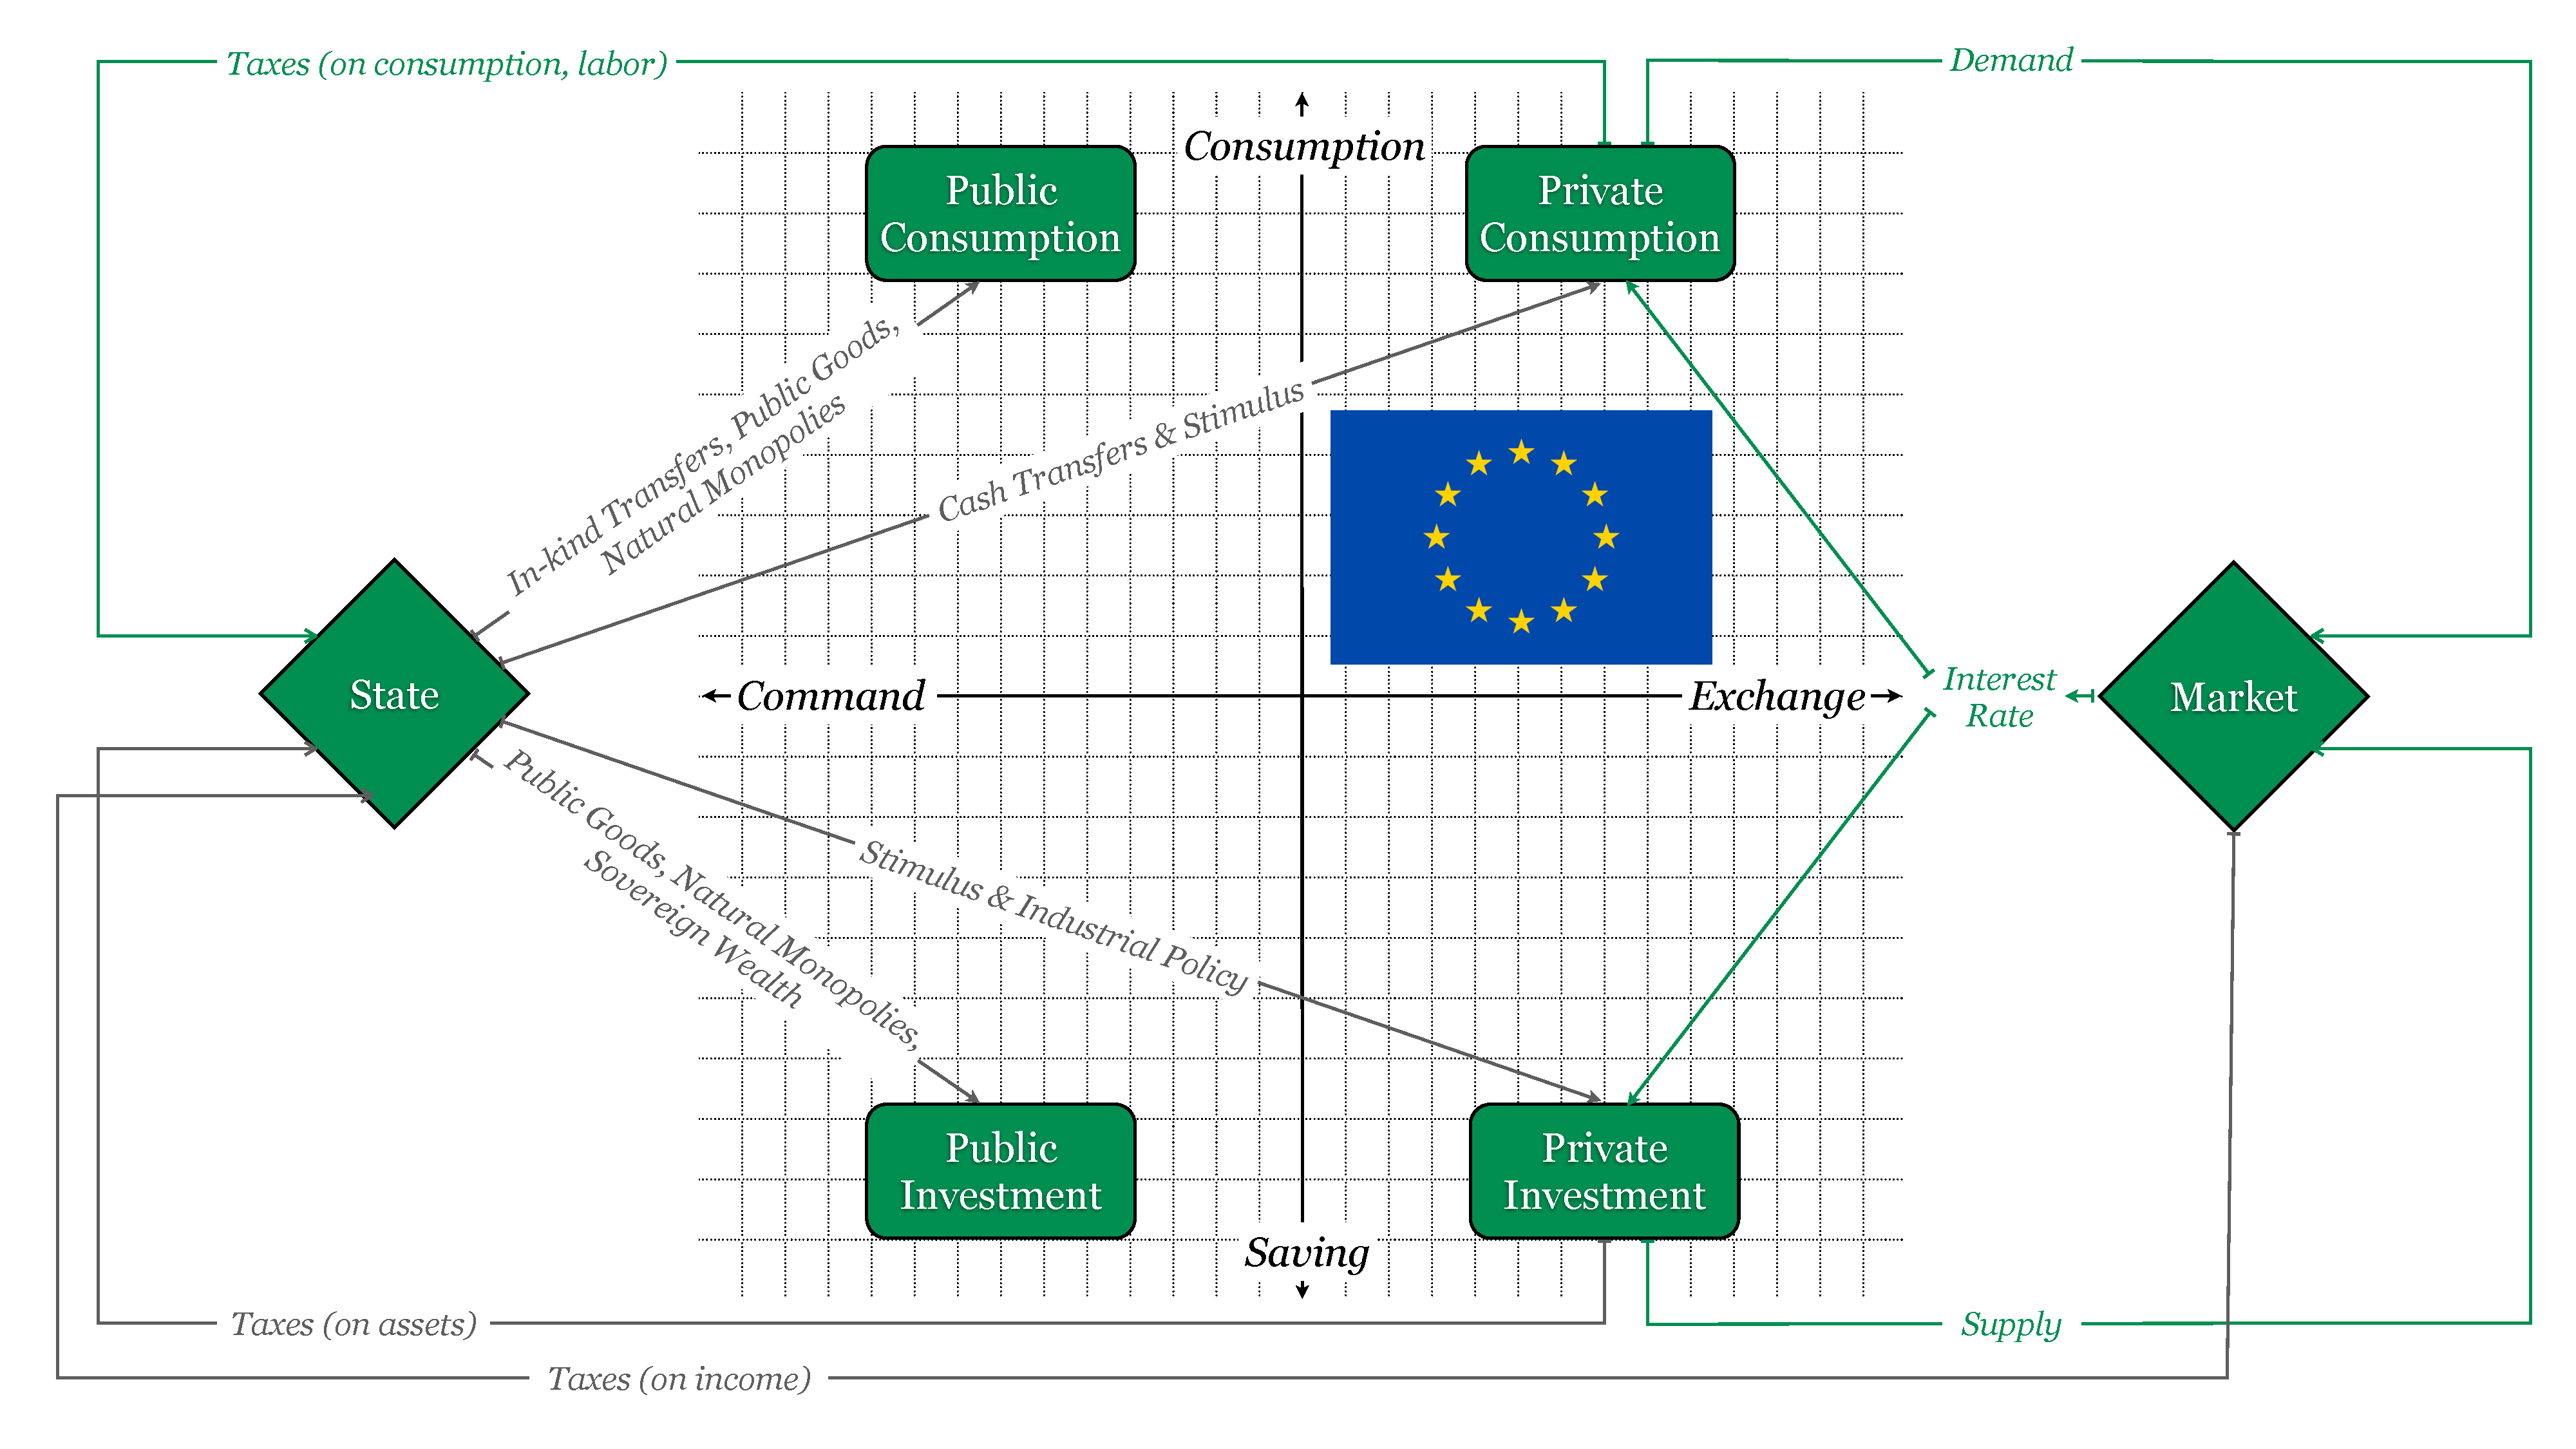
\includegraphics[width=1\textwidth]{coordinate-space-constrained}  
	\caption{Constrained Coordinate Space of a Dysfunctional Mixed Economy}
	\label{fig:coordinate-space-constrained}
	\end{center}
\end{figure}

By its dysfunctional design, the european mixed economy yields ever more to markets while the other part of the mixed economy, the state, is on the retreat. Bereft of their old, flexible and capable social contracts, the acquis will, nay, already \emph{has} --- however fortuitously --- remade european society in the neoliberal, consumerist image. ``Neoliberalism'' and ``consumerism'' are, in this case, not catch-all labels of disaffection, but I choose them with equal anger and care, and they apply precisely. The aquis is:
\begin{description}
	\item[Neoliberal,] because, eviscerating the state, it morphs markets from one of several \emph{means}, to inescapable \emph{reality} or even ultimate \emph{end}, neither of which it is, nor should be.
	\item[Consumerist,] because, it cannot set a positive savings rate, and leaves austere members no choice but to loot real savings, and give into the temptations of bubbles. As a result, much of the resources of the communal household will be devoted to near-term consumption\footnote{
		The \gls{EU} commission is quite explicit about this:
			\begin{quote}
				\emph{``The Single Market Review put \emph{(sic!)} citizens, consumers and \glspl{SME} at the centre of policy-making.''}\\
				--- \citealt{Commission2008}: 3	 
			\end{quote} 
		One wonders, at least, why, in addition to \emph{citizens}, consumers and \emph{some} (though not other) firms are also mentioned, when, in a functioning market, the latter two should be served only as proxies of the ultimate beneficiary, the citizen.}.
	
\end{description}

Just how angelic the postwar mixed economy really was, I do not know\footnote{
	To mention just a few red flags, it is unclear what costs Postwar prosperity extracted from others (dependence or world systems theory), we do know whether or how Western affluence can be repeated without the same gigantuan carbon footprint and we worry whether broad-based growth in value-add is but a historical episode (cost disease).}. 
Still, \emph{relative} to 19th century mass poverty \citep{MarxEngels-1848-aa}, 20th century ``mob politics'' (\citealt{Crouch2004}: 158) and the spectre of 21st century neo-laissez-faire, the mixed economy, and the welfare state it has enabled, appears as singular achievements of the modern era. The economic institutions of Postwar Western Europe have brought about unseen prosperity and equity, all in relative peace and freedom. 

That is an old deal worth fighting for.

\subsection{Catch-Up}
\begin{quote}
	\emph{``Three tomatoes are walking down the street --- a poppa tomato, a momma tomato, and a little baby tomato. Baby tomato starts lagging behind. Poppa tomato gets angry, goes over to the baby tomato, squishes him, and says: catch up.''} \\
	--- \href{http://www.youtube.com/watch?v=5D-QKY0-Bxk}{Mia Wallace in Pulp Fiction (1994)}
\end{quote}

Too easily, discontent with a retrenching Western European welfare state blames \gls{CEEC} for ``social dumping'' %source
or otherwise slides into poorly disguised economic nationalism. 
It must not: whoever thinks that Western and Northern, otherwise intact mixed economies now whither away because of competition from the East and the South, misunderstands, or --- more likely --- misconstrues the issue.

Of course, the newly opened, low-productivity and low-capital markets in the poorer East and South have much lower, often proportional taxation, especially on capital incomes. They \emph{cannot} afford high, or progressive taxes on capital, if they are to remain competitive, let alone converge\footnote{
	For example, L\'{a}szl\'{o} Kov\'{a}cs (2004), then Commissioner for Taxation and Customs asked that tax rates must be allowed to differ 6-8\% simply to make up for the remote location of some markets.} 
Had Romania the capital income taxation of pre-reform Sweden, the net returns on any investment would fall tremendously. Given the low labor and total factor productivity in Romania, an investment might not be profitable at all, and capital might instead stay in high-tax, but also high-productivity Sweden. Romania would not be able to attract much foreign capital, which it so direly needs to leapfrog into convergence.
	
By contrast, the high-productivity, high-capital markets in the West and North, \emph{could} afford higher, and more progressive taxes, if only they did not face tax competition from all other \gls{MS}. Had Sweden the capital income taxation of post-accession Romania, or even the 0\% \gls{CIT} of non-member Moldova \citep{Piatkowski2008}, it would have to abandon much of its mixed economy. Forced to finance its large public sector only out of labor, or other immobile, proportional sources, the tax wedge on the lower and middle strata of society would become unbearable. %add \href

At first sight, there appear to be only two policy responses to this conundrum:
\begin{enumerate}
	\item \emph{High European-Level Taxation.} \gls{MS} might agree to enforce union-wide, uniformly high and progressive taxes on mobile bases, that would save welfare in the rich \gls{MS}, but at the cost of laggard growth in the poor capital-deprived \gls{MS}. Such tax cooperation would save the welfare state, but sacrifice fast, or even any, convergence.
	\item \emph{Tax Competition.} \gls{MS} might continue with the status quo ante, set tax rates individually and let competition whither away levels and progressivity. Such tax competition would sacrifice the welfare state, but bring some convergence ``through the back door'' as rich \gls{MS} capital will to rush to poor \gls{MS}: poorer (and smaller) countries win under tax harmonization, as evidenced by their opposition to even nascent \gls{EU} tax cooperation (\citealt{Kellermann2009}: 138)\footnote{
		Capital inflows will be particularly effective in relatively poor economies. As these economies, supposedly, still lie far below the golden rule of saving \citep{Solow1956}, returns on capital will be much higher than in richer economies where further (near-Solowian) capital deepening faces diminishing returns (for example, \citealt{Barro1995} or \emph{ibid.} 1992 as cited in \citealt{Beckfield2009}: 3).}.
\end{enumerate}

Such are the alternatives that politicians might peddle, pitting poor members against rich, convergence between them against welfare within. These are, as so often in defunct mixed economies, impossible choices to make, seemingly forcing European democracies to play a game of zero-sum.

Alas, regional economic integration, as all trade, is not zero-sum game: there are gains to be had, if not accruing to everyone equally. Sweden is better of for having a prospering, converging Romania as a trading partner, with different absolute or comparative advantage, capital endowments and areas of specialization. Out of the proceeds of this positive-sum game, there is a third option:
\begin{enumerate}
	\setcounter{enumi}{2}
	\item \emph{High European-Level Taxation With Side Payments.} \gls{MS} agree to enforce union-wide, uniformly high and progressive taxes on mobile bases, but rich \gls{MS} recompense poor \gls{MS} for their ensuing competitive disadvantage. Absent different taxes rates on mobile factors, the union as a whole is able to choose freely amongst the trade-offs of a mixed economy, including a well-funded welfare state. Still facing low labor productivities, poor \gls{MS} receive fiscal transfers that they can use to build capital stock, educate their workforce, upgrade infrastructure, or even subsidize investment. For example, poor \gls{MS} might lower or even abandon taxation of some or all immobile factors, such as low-productivity labor. Facing a small or no tax wedge, maybe even receiving subsidized or free health care, or some other \gls{NIT} of sorts, the low-productivity workers in poor \gls{MS} would be able to accept yet lower gross market wages, and become competitive again, even as investors have to pay high taxes\footnote{
		To remind readers that this is not, in fact, what the acquis currently stipulates: The overall structural and cohesion funds for 2007--2013 amount to no more than \euro{} 347 billion, less than 3 times the budget of the city of Berlin (\euro{} 21 billion in 2009), or about 0.005 \% of the budget of Germany (\euro{} 1,164,000 billion in 2011). In addition, \gls{EU} budget negotiations are still marred by \emph{juste retoure} attitudes, with \gls{MS} wanting to get paid out what they have received --- the very opposite of a redistributive regime (for example, \citealt{Begg2008a})}.
	
	Side payments need to be initially large enough but decrease over time, and they must be used wisely by poor \gls{MS}. As in any subsidy or  protection, it will be difficult to avoid long-term dependence and rent-seeking.
	
	If we get it right, though, high european-level taxation with side payments will save the mixed economy, enable a potent welfare state, clear factor markets, converge living standards in the union and keep us all on the long-term growth path. 
\end{enumerate}

%add game theory here. Is there a game to be played? %create a table about the options in the catch-up game.

We need not trade off openness and convergence \emph{between} \gls{MS} with efficiency and equity \emph{within} them. In fact, they are the same issue: behind the pressures on rich welfare states always lurks the question of convergence: just how fast, and by which means, do we want the poor members to catch up?

If we opt for policy response \begin{inparaenum} 
	\item high european-level taxation, convergence will be minimal and through the market only. If \item we choose tax competition, convergence will be faster, and still only market-led. If we \item adopt high european-level taxation with side payments, convergence can progress at an arbitrary speed, with a substantial state component. \end{inparaenum}

Deciding on the speed of the catching up may just be the deeper question of european integration that many politicians of all colors, but especially those tending to economic nationalism, may seek to avoid by misrepresenting european choice in dichotomous terms of more or less protection, more or less integration. Convergence supported by side payments \emph{does}, of course, include a zero-sum component, as any redistribution by definition does. 

But it is not, as it is easily made out to be, redistribution \emph{between} one economy and another, it is instead, redistribution \emph{within} one, European economy. Whenever the markets expand beyond borders, so, too, the abstractions of the mixed economy rule at a higher level, and they apply not just to tax --- the clearest case that I have here illustrated --- but to all command interventions prone to arbitrage: as the first good, service, or capital equipment crosses the border, the two trading partners have already adopted \emph{one} of the three regimes of economic integration, and, related, have made their however implicit choice of just how, and how fast, the poorer party gets to catch up.

The elephant in the room of european economic integration is this: if we are to save the mixed economy, we have to explicitly decide, not just agree by default, how fast we want to converge \footnote{
	It too, is neither new nor revolutionary: internally heterogenous mixed economies have always, with varying results, dealt with this question. In the US, much of the controversy about the role of the federal government boils down to the question of how much rich Texans should dole out to poor Louisianans. In Italy, the rift is between North and South (for example, \citealt{PutnamLeonardi-1993-aa}) and in Germany, initially between industrial and rural states, since 1990 between old and new \emph{Laender}.}.

%On the old deal: the imbalances and dysfunctions of the potent mixed economy provide fuel for the cyclical, and now fairly grave fin market crises. Without this fuel, these crises would not build. But, they are not the only problem, nor are they the only thing we should fixate on in avoiding crises. We also need macro prudential oversight and regulatory intervention to fight the market failures that lie at the heart of financial crises.
	
%\section{So, you Want a Revolution?\ldots} \label{sec:Revolution}

%\begin{quote}
%	\emph{So, you want a revolution?\\*
%	Well, you know: 
%	We all want to change the world.}\\*\\*
%	The Beatles (1980)
%\end{quote}

%Yes, the PCT would be a revolutionary overhaul of tax, redistribution and economic production. But no, this is not socialism, or anything of the kind. Even if I have my way, there will still be \hyperref[des:Entrepreneurship]{private ownership of the means of the production}. And there should be, as per desideratum \ref{des:Entrepreneurship}.

%But still, this is a normative project as much as it is an analytical project. It is as much policy as it is social science. I do not want to apologize for that. 

%After two years of studying at the \hyperref[http://www.hertie-school.org]{Hertie School of Governance}, \hyperref[http://maxheld.de/2009/10/13/setting-goalposts/]{``disinterested'' just does not cut it anymore}. If social science and policy analysis does not want to end up being latently affirmative, it should start asking the status quo a little harder, and a little more creative questions.

%Here is one.

%\subsection{The Fierce Urgency of Taxation} Tax is not boring, and tax is not inconsequential. In fact, ``tax represents the last battle line for any meaningful redistribution of material resources from the better able to the least well off'' (\citealt{McCaffery2005}: 936). 

%We should be grateful that this last battle line lies in the abstractions of tax, and is no longer violently fought in revolutionary strife. 

%But this last battle line must not be abandoned, nor retrenched. Much is at stake. With a defunct fiscal configuration, our polity is paralyzed. For, as the conservative Edmund \citeauthor{Burke1790} remarked, ``[t]he revenue of the state \emph{is} the state'' (\citeyear{Burke1790}: 111, emphasis added.). 

%The PCT was first suggested in the 1940s, to curb inflationary tendencies in a time when government expenditure \emph{could} not be reduced (\citealt{Cheng1953}: 333). The United States were at war, everywhere against the axis powers, later, in Korea, then in a Cold War of hemispheric scale. The American polity needed greater saving, and more public goods (defense, after all, is the quintessential public good). 

%My point is this: we are \emph{there} again. With no war, at least on our continent, but with widespread unemployment, lagging growth, rampant social problems, an education with too little, too unequal opportunity for many, and a planetary system thoroughly out of balance --- we are \emph{there} again.

%The Progressive Consumption Tax returns to the polity, what is hers: the ability to democratically decide how much we want to save for our children, how large the sticks and carrots should be today, how we want the economic pie to be sliced, and what we want it to be used for. Let us reclaim that enlightened emancipation: that really, how we live together \emph{is} of our own, collective choosing. \emph{That} is the project of the \hyperref[http://www.policy-net.org/blogs/thepotentpolity]{potent polity}, to which I here wish to contribute.

%These are no abstract considerations. Right beneath the surface of tax lie the life chances of people. The immigrant schoolgirl in Berlin-Kreuzberg, who needs her public school to be a palace of learning and self-fulfillment. The management consultant who did not make the promotion, and cannot afford the luxurious trip to the Seychelles with his girlfriend. The cancer patient who needs her disease to be better understood, and cured. Our polity's ability to tax, to finance and to redistribute makes all these lucks, and all our luck, too.

%To live up to the potential of our progress, and to honor the promise of our democracy we must reunite what \emph{is not} antithetical: rigorous competition, high productivity, a well-equipped polity and robust redistribution. 

%If we get tax right, we can have it all: ``to prosperity and opportunity'', indeed.

\section{Why Tax Matters to Democracy}

\begin{quote}
	\emph{``But who can say how much is endurable, or in what direction men will seek at last to escape from their misfortunes.''}\\*
	--- John Maynard \cite{Keynes1936}
\end{quote}


\begin{quote}
	% "I'm still trying to climb out from under the avalanche of horror, nightmare and disgust that all of this [the 2011 US debt ceiling crisis] dumped on me, along with, I suppose 300 million other Americans and it's a little hard to sort out your thoughts after this much awfulness comes along. [...] Sorry but I actually do think that this [the 2011 US debt ceiling crisis] is one more symptom of a long, slow constitutional crisis, it goes back further than the 2000 election. This kind of thing keeps happening again and again, it's as if our system is getting hardening of the arteries, we get a stint once in a while [...] but to me it's getting scarier and scarier over the long haul. [...]
	\emph{``There are a lot of rational (tax) ideas out there, there are a lot of ways you could build something from scratch that would look roughly like the society we have now, but would work better, would be smoother and fairer and all that. And of course, these things are proposed in politics [...] and then they cannot be done. Then our system prevents them from happening or garbels them in such a way that they look supremely ugly, once they are created [...].This is a machine for creating disillusionment with government, cynicism, Tea-Partyism, and over time, this is our county, our democracy eating itself alive. [...] And that's why I get a little discouraged sometimes."}\\
	--- Hendrik Hertzberg (2011) on The New Yorker podcast \emph{The Political Scene}
\end{quote}

%(Both of this is Foreword ix, in Esping-Andersen 2002)	
	%“The irony (of structural transformation and existing welfare programmes) is that class may be less visible, but its importance is arguably far more decisive. (…) The post-war welfare state no doubt succeeded in equalizing living conditions, but it failed to deliver on its promise of disconnecting opportunities from social origins and inherited handicaps.” (ibid: 3)
	% This I like, a lot: “(…) there is a very good argument that equality of opportunities and life chances is becoming sine qua non for efficiency as well.”	
	%	-         “de-familialization” is an ugly word, but necessary nonetheless.

%Not sure I agree with crouch that we want back the class in itself working class, that may be misconstruing the past and we don't really want that today. Think about that. Also note that even crouch misunderstands the taxation of firms.

%Cite Eliasoph on why we need a big ass issue; not a small scale issue. You're leading to despondence. Quote early passages of Eliasoph. Also argue with Eliasoph "Charles said …" that by all means trying to CHANGE things, and only discuss things you can change, has drawbacks.

%[ ]  also: markets are an incentive-driven form to organize activity. This is all good and well, but an incomplete view of the ability of humans to produce. The deliberative model is another way to do this. It's kind of the synthesis: it abandons rational motivation, but it still features the abstractions that govern complex, rich socieities.

%from europe piece

%Cite Young's critique of deliberation as support for "hypothetical".

\section{The Social Contract}
%---
%Martin, I. W., Mehrotra, A. K., & Prasad, M. (2009). The Thunder of History - The Origins and Development of the New Fiscal Sociology. In I. W. Martin, A. K. Mehrotra, & M. Prasad (Eds.), The New Fiscal Sociology - Taxation in Comparative and Historical Perspective. Cambridge, UK: Cambridge University Press.
	%1: "In the modern world, taxation is the social contract."

%here comes another copy/paste from the europe piece

Crucially, we must, again, understand that economic integration must always beget more economic and political integration, that, production at great economic scale implies solidarity at the same scale.

\emph{That} is the story of economic integration and material progress. Living on a scarce and harsh planet, for which, alone, we are ill-equipped, we escaped the \citeauthor{Malthus1798}ian curse of overpopulation and starvation by scaling up our production. That is, to this day, how we remake an arithmetically growing material world, to feed our geometrically growing hunger: we join forces to bend upward the production curve, and wrest from it above-linear returns. To reap such economies of scale, in agriculture \citep{Diamond1997}, in the production of violence \citep{Tilly-1985-aa}, or in europe-wide automotive engineering \citep{Krugman-1980-aa}, we have to master the feat of cooperation in the face of atomistic incentives. Akin to ever-increasing entropy, the arrow of pre-historic organic life, and history of human life on earth progresses by increasing complexity, specialization, but also, always, mutual dependence. \citeauthor{Wright1994} thus describes the transformation of individual cells into higher organisms: they become richer, more resilient, but they must also sacrifice, and will do so only to the extent that they have successfully merged their genetic instructions (\citeyear{Wright1994}: Chapter 7, 8). %better double-check this stuff. This isn't quite right yet.

And so it is with european, or other regional economic integration: opening up commerce to one common market makes everyone richer by the magic of comparative advantage --- if not necessarily by the same amount. But, if this association is to remain stable, some other elements of human organization have to follow to that higher level, if they are not to perish and destabilize. In the \gls{EU}, continent-wide commerce also requires continent-wide taxation, regulation and monetary policy, if the formerly stable and re-productive system of a mixed economy is to remain operative.

The genius of the otherwise hyper-federal, and hyper-liberal US Constitution is that it foresees this functional necessity in its commerce clause\footnote{
	\ldots the reach of which was only recently discussed in the 2012 US Supreme Court ruling on the Affordable Care Act.}.
It stipulates that, precisely as commerce traverses the otherwise autonomous states, the federal polity asserts itself. The German constitution knows a similar norm:

\begin{quote}
	\emph{``The Federation shall have the right to legislate on matters [\ldots] if and to the extent that the establishment of equivalent living conditions throughout the federal territory or the maintenance of legal or economic unity renders federal regulation necessary in the national interest.''}\footnote{
		In the German original:
			\begin{quote}
				\emph{``Auf den Gebieten [\ldots] hat der Bund das Gesetzgebungsrecht, wenn und soweit die Herstellung gleichwertiger Lebensverhältnisse im Bundesgebiet oder die Wahrung der Rechts- oder Wirtschaftseinheit im gesamtstaatlichen Interesse eine bundesgesetzliche Regelung erforderlich macht.''}\\
				--- Grundgesetz der Bundesrepublik Deutschland: Artikel 72, Absatz 2 (Bonn, 1949)
			\end{quote}}\\
	--- Basic Law for the Federal Republic of Germany: Article 72, Paragraph 2 (Bonn, 1949)
\end{quote}

It too, displays the same genial insight into the relationship between economic and political integration: as the commerce clause, it does not compel any particular social or other policy, but, if economic integration has occurred, endows the democratic sovereign to rule at the newly emerged, higher level of societal organization.


%some of the following will have to go
\section{Growth and Solidarity} \label{sec:growth-solidarity}

\begin{quote}
	\emph{``The Congress shall have Power [...] To regulate Commerce with foreign Nations, and among the several States, and with the Indian tribes''}\\
	--- Constitution of the United States: Article I, Section 8, Clause 3\footnote{
		Known as the commerce clause.} 
	(Philadelphia, 1787)
\end{quote}

Let me now return to the first order perspective: what, from here, is to be done about european integration and its failing welfare states?

Crucially, we must, again, understand that economic integration must always beget more economic and political integration, that, production at great economic scale implies solidarity at the same scale.

\emph{That} is the story of economic integration and material progress. Living on a scarce and harsh planet, for which, alone, we are ill-equipped, we escaped the \citeauthor{Malthus1798}ian curse of overpopulation and starvation by scaling up our production. That is, to this day, how we remake an arithmetically growing material world, to feed our geometrically growing hunger: we join forces to bend upward the production curve, and wrest from it above-linear returns. To reap such economies of scale, in agriculture \citep{Diamond1997}, in the production of violence \citep{Tilly-1985-aa}, or in europe-wide automotive engineering \citep{Krugman-1980-aa}, we have to master the feat of cooperation in the face of atomistic incentives. Akin to ever-increasing entropy, the arrow of pre-historic organic life, and history of human life on earth progresses by increasing complexity, specialization, but also, always, mutual dependence. \citeauthor{Wright1994} thus describes the transformation of individual cells into higher organisms: they become richer, more resilient, but they must also sacrifice, and will do so only to the extent that they have successfully merged their genetic instructions (\citeyear{Wright1994}: Chapter 7, 8). %better double-check this stuff. This isn't quite right yet.

And so it is with european, or other regional economic integration: opening up commerce to one common market makes everyone richer by the magic of comparative advantage --- if not necessarily by the same amount. But, if this association is to remain stable, some other elements of human organization have to follow to that higher level, if they are not to perish and destabilize. In the \gls{EU}, continent-wide commerce also requires continent-wide taxation, regulation and monetary policy, if the formerly stable and re-productive system of a mixed economy is to remain operative.

The genius of the otherwise hyper-federal, and hyper-liberal US Constitution is that it foresees this functional necessity in its commerce clause\footnote{
	\ldots the reach of which was only recently discussed in the 2012 US Supreme Court ruling on the Affordable Care Act.}.
It stipulates that, precisely as commerce traverses the otherwise autonomous states, the federal polity asserts itself. The German constitution knows a similar norm:

\begin{quote}
	\emph{``The Federation shall have the right to legislate on matters [\ldots] if and to the extent that the establishment of equivalent living conditions throughout the federal territory or the maintenance of legal or economic unity renders federal regulation necessary in the national interest.''}\footnote{
		In the German original:
			\begin{quote}
				\emph{``Auf den Gebieten [\ldots] hat der Bund das Gesetzgebungsrecht, wenn und soweit die Herstellung gleichwertiger Lebensverhältnisse im Bundesgebiet oder die Wahrung der Rechts- oder Wirtschaftseinheit im gesamtstaatlichen Interesse eine bundesgesetzliche Regelung erforderlich macht.''}\\
				--- Grundgesetz der Bundesrepublik Deutschland: Artikel 72, Absatz 2 (Bonn, 1949)
			\end{quote}}\\
	--- Basic Law for the Federal Republic of Germany: Article 72, Paragraph 2 (Bonn, 1949)
\end{quote}

It too, displays the same genial insight into the relationship between economic and political integration: as the commerce clause, it does not compel any particular social or other policy, but, if economic integration has occurred, endows the democratic sovereign to rule at the newly emerged, higher level of societal organization.

%add more from the Papier debate here?

What the \gls{EU} needs, is not more stringent subsidiarity, but it's inverse: a commerce clause.

%here used to be \ref{sec:LD-Difference} part, now only in better democracy

%\subsection{Postwar}

%\begin{quote}
%	\emph{``Meanwhile [in 1989], across the Leitha and Danube rivers just a few kilometres to the east, there lay the ‘other' Europe of bleak poverty and secret policemen. The distance separating the two was nicely encapsulated in the contrast between Vienna's thrusting, energetic Westbahnhof, whence businessmen and vacationers boarded sleek modern expresses for Munich or Zurich or Paris; and the city's grim, uninviting S\"{u}dbahnhof: a shabby, dingy, faintly menacing hangout of penurious foreigners descending filthy old trains from Budapest or Belgrade.''}\\
%	--- Tony \citeauthor{Judt2006} (\citeyear{Judt2006}: 5)
%\end{quote}

%!marginpar
%\marginpar{Because this section is so small and I have so little to say on it, it might better go. I just love the Judt quote.}

%In his epic Postwar tome, \citeauthor{Judt2006} chronicles the divergent paths that drove apart eastern and western Europe, as the post-war settlement inflicted on them the historical accident of Cold War division. The wounds of this continental tear have not healed, in fact, until and unless we install democratically governed, intact mixed economy on the continent, it will continue to pain and undermine the union, only superficiously covered by the paltry Band-Aid of the common market.

%If there is a Postwar history to building welfare states in \gls{CEEC} is that so far, they will only succeed if we finally close the tear of 40 years of state socialism, and agree on how fast to have the East catch up, and how to make it happen. 

\subsection[Weimar]{Weimar}

%via MPP on inefficient inequality
	%\paragraph{Extreme Inequality May Lead to Instability, Threaten Democracy} 
	%this might have to go somewhere else. This is in the wrong place.
	%Democracy and peaceful resolution of societal contradictions have emerged in tandem with economic growth \emph{and} redistribution \citep{Marshall-1950-aa}. There are empirical findings that suggest that this link may still operate today. The political sociology of modernization theory suggests that economies, political institutions and mass values evolve \emph{together}, in a project of ever increasing human emancipation \citep{InglehartWelzel-2005-aa}. These links hold both at the societal and at the individual level: more materially affluent people are more likely to hold pro-democratic mass beliefs, including generalized trust \citep{KnackKeefer-1997-aa}, tolerance, and self-actualization \citep{InglehartWelzel-2005-aa}. Other, structural(ist) formulations of this link stress the importance of \emph{cross-cutting cleavages} for functioning democracy \citep{LipsetRokkan-1967-aa}. 

%\begin{quote}
%	\emph{``There’s a storm coming, Mr. Wayne. You and your friends better batten down the hatches. Because when it hits you’re all going to wonder how you ever thought you could live so large and leave so little for the rest of us.''}\\
%	--- Selina Kyle (``Catwoman''), Dark Knight Rises (2012)
%\end{quote}

\begin{quote}
	\emph{``But who can say how much is endurable, or in what direction men will seek at last to escape from their misfortunes''}\\
	--- John Maynard \cite{Keynes1936}
\end{quote}

Optimists, not just of the Panglossian kind, are always inclined to see glasses half-full, and so many argue that any, even imperfect or negative European integration is better than none.  That is not so much optimistic, as it is hopelessly naive. The metaphor is flawed. Societies are not just glasses half-full or half-empty, they are dynamic systems, residing within, and reproducing the walls of this glass: half-\emph{built} glasses, as the \gls{EU} defunct mixed economies, are not merely waiting to be filled, they can also drain of all remaining water, or topple and fall over.

The democratically governed mixed economy is \emph{the} institutional achievement of the century, and as a social compact, it is fragile. As \citeauthor{Offe2003} points out, ``it is much more likely that a European-styled [mixed economy] capitalism transformed itself into a liberal model'' than the other way around, or, appropriating Lech Walesa, ``it is easier to make fish soup out of an aquarium than the other way around'', because it --- like the mixed economy --- depends upon ``supportive dispositions of a cognitive as well as moral kind'' (\citeyear{Offe2003}: 446). A mixed economy, as the democracy that governs it, is ``easily lost, but never finally won'', as the first African-American federal judge William H. Hastie ominously warned. 

We have already lost much of the mixed economy, and we are now risking to harm or loose democracy, too: not just democratic rule \emph{of} the \gls{EU}, but democracy \emph{in} Europe, too (\citealt{Scharpf1997}: 19).

Democracy needs not just a legitimacy of inputs, but also of outputs (on Europe see \citealt{SchaGove1999}). In \citeauthor{Dahl-1994-ab}'s (\citeyear{Dahl-1994-ab}) terms, democracies need to be ``system effective'', in \citeauthor{Zurn-2000-aa}'s \citeyearpar{Zurn-2000-aa} apt words, democracies need to be ``output congruent'': people must be able to choose any (liberal) policy they want to govern a given polity. The \gls{EU}, currently violates output congruency: with an impotent, largely defunct mixed economy, the people of Europe cannot have all materially possible policies to improve their currently grim life chances, including crushing trade imbalances, demoralizing structural unemployment, wild economic cycles, public squalor and rampant inequality. In the half-built, supposedly \emph{sui generis} glass of Europe, there is a wide mismatch between the two walls: the exchange components of the mixed economy roam the continent, while most of the command components are confined to the constrained nation state. As a result, the glass is heavily leaking water, both in efficiency and equity.

Over time, the hardship that this arrangement inflicts on people, especially in the poorer, more austere \gls{MS} (Greece), and when the imbalances and crises unload (Spain, Ireland), will corrode the inputs of popular rule, too, and fray the social contract. \citeauthor{Offe2003} has already seen the grave-diggers of liberal democracy, capitalizing on the resulting popular discontent of such ``permanent austerity'' \citep{Streeck2010c}: 
\begin{quote}
	\emph{``Also, a third voice, luckily with much less resonance, is making itself increasingly heard in European politics, a voice which claims that the social security of workers (as well as the protection of citizens from violent crime), on the one hand, and efficiency of production and competitiveness, on the other, can only be reconciled if national borders are sealed to the influx of foreign people, foreign workers, foreign goods, and those praying to `foreign' gods. Since the mid-1990s, integrating Europe has seen the sometimes sudden and spectacular rise to electoral success of figures such as Pia Kjaersgaard (Denmark), Umberto Bossi and Gianfranco Fini (Italy), Pim Fortuyn (Netherlands), with Jean Marie Le Pen (France), J\"{o}rg Haider (Austria) and Carl Hagen (Norway) being among the pioneers of this new field of populist political entrepreneurship. Le Pen has described himself in the 2002 French electoral campaign as being a leftist in social affairs, a rightist in economic affairs, and a nationalist for everything else. This formula, which is designed to resolve the tension between liberal market freedom and welfare state status rights by ethno-nationalist, xenophobic, and anti-European appeals, is applied by his rightist populist colleagues as well."}\\
	--- \citeauthor{Offe2003} (\citeyear{Offe2003}: 454)
\end{quote}

The ground of popular resentment will only grow more fertile as the Euro crises goes on. The crippling economic depressions of the south, and the ever-insufficient, multi-billion bail-outs from the north are political dynamite, waiting to be ignited by fringe populists. 

If the extreme right, or extreme left, and/or nationalists start playing with this fire, the moderate voices of social democracy, liberalism and conservativism will have little to douse the flames, because in fact, both the polities in the north and south \emph{are} faced with thoroughly unattractive alternatives.

In the now often wretched south, policy makers must either accept the conditional straightjacket imposed by the \gls{EU} and its rich sponsors, or jump the cliff of secession and sovereign default, all but ensuring all-out economic collapse under autarky. In the still largely isolated north, policy makers must either continue to periodically support often (but not always) failing governments in the south to alleviate the gravest imbalances, or splinter the union and forego the years, maybe decades of economic growth that wide integration brought.

European democracies thus are also no longer \emph{input congruent} \citep{Zurn-2000-aa}, in addition to the already grave, but homemade democratic deficit of a heavily intergovernmentally-biased institutional setup. Faced with such non-alternatives, the people of Europe are no longer subjected only to decisions in the making of which they had a say. For the past two years, every couple of months, German or Greece executives, legislators and voters are asked to choose between bail-out or break-up, austerity or abyss, always at gunpoint, with the entire european project held hostage (for example, \emph{Grexit}, followed by Portugal, Spain, Italy, followed by doomsday). If the people of Europe merely get to choose between a rock and a hard place, popular sovereignty becomes a farce.

\citeauthor{Offe1998}'s \citeyear{Offe1998} intuition is, tragically, fully borne out:	
\begin{quote}
	\emph{[\ldots] that every interim solutions between the extremes of intact national sovereignty on the hand, and complete european supranationalty of a European Federation will, inevitably, violate both the reference point of welfare state protection and that of democratic legitimacy.}\footnote{\label{fn:Offe-regress}
		In the German original:\\
		\begin{quote}
			\emph{``Meine These ist, dass jede Zwischenl\"{o}sung, die zwischen diesen beiden Extrempolen intakter nationalstaatlicher Souver\"{a}nit\"{a}t einerseits, einer kom-plettierten europ\"{a}ischen Supranationalität in der Gestalt eines föderalen eu-ropäischen Staates andererseits gefunden wird, zwangsl\"{a}ufig beide Be-zugswerte verletzt, den des wohlfahrtsstaatlichen Schutzes ebenso wie den der demokratischen Legitimation. Demnach k\"{o}nnte man im Blick auf die europäische Integration einen Abstieg auf jener Leiter vermuten, die T. H. \cite{Marshall-1950-aa} sich als Modell für den Prozess der europ\"{a}ischen politischen Modernisierung vorgestellt hat. Die drei Stufen dieser Leiter sind bekanntlich die kumulative Durchsetzung liberaler, demokratischer und sozialstaatlicher Rechte. Die Frage ist, ob im Prozess der europäischen Integration die demokratische und die sozialstaatliche Stufe in r\"{u}ckw\"{a}rtiger Richtung passiert werden und im Ergebnis der Euro-B\"{u}rger allein mit der Rechtsausstattung eines (neo-)liberalen Marktteilnehmers dastehen wird.''}\\
			--- \citeauthor{Offe1998} (\citeyear{Offe1998}: 41)\\
		\end{quote}}
	--- \citeauthor{Offe1998} (\citeyear{Offe1998}: 41)
\end{quote}

The political fringes will prosper, as they exploit these violations, both from the extreme left and the extreme right. The extreme left will fan the flames of societal disintegration by pitting liberal freedoms --- especially those of property and contract! --- against welfare protection and democratic sovereignty. Merely a change in tone, the extreme right will push societal regress by pitting all cosmopolitan integration and solidarity against always national welfare and sovereign rule. This new game is rigged against liberal democracy and the moderate voices (or cross-cutting cleavages, \citealt{LipsetRokkan-1967-aa}) on which it so thoroughly depends. 

What the glass-half-full-optimists forget is that societal, political and economic integration can reverse course, too. The self-reinforcing dynamics of integration operate in \emph{both} directions: more integration begets more integration (as Monnet had hoped, according to \citealt{Schmitter1999}: 948), but regress also begets more regress. As a matter of fact, the neo-functionalists are right, if one-sided (Tranholm-Mikkelsen 1991 as cited in \citealt{Bieler2003}: 1)

The course of economic disintegration is quite clear: literally the milli-second that an over-indebted \gls{MS} is thought to leave the \gls{EMU}, anticipating massive devaluation, all holders of cash in, say, Greek institutions, will take their money out\footnote{
	In fact, the run on Greece is already underway, with the country having lost almost a third of its domestic bank deposits by May 2012, according to \cite{TheEconomist2012}.}. 
Faced with such an economy-wide bank run, the Greek government will be forced to install capital controls, effectively leaving the common market. Without international finance, the remaining trade, too, will be greatly constrained. Just the credible rumor of \emph{Grexit} could, thereby, almost in an instant, unravel 21 years of integration since the country joined in 1981.

We tread the course of political disintegration if --- outflanked by populists --- our \gls{MS} democracies increasingly re-embrace the supposed trade-off between national interest and political unification, and again entertain the nationalist politics that the union was built to overcome, in a scenario of decay similar to that painted by \citeauthor{BeckGrande-2007-aa} (\citeauthor{BeckGrande-2007-aa}: 339ff, or \citealt{Schmitter1999}: 947).

Writ large on society, this is the disintegration that \citeauthor{Offe1998} presciently feared in \citeyear{Offe1998}:
\begin{quote}
	\emph{[\ldots] one could suspect a downward descent on the ladder that T. H. \cite{Marshall-1950-aa} suggested as a model for european political modernization. The three rungs on this latter are the cumulative expansion of liberal, democratic and social rights. The question is, whether during the course of european integration, we will pass the democratic and welfare state stages on our way down, and, as a result, european citizens will be equipped merely with the rights of a (neo-)liberal market participant.}\footnote{
		For the german original, see footnote \ref{fn:Offe-regress}.}\\
	--- \citeauthor{Offe1998} (\citeyear{Offe1998}: 41)
\end{quote}

We have been here before: 1918. Torn apart by nationalist antagonisms and frayed by beggar-thy-neighbor responses to depression, economies \emph{can} disintegrate, as the havoc-wreaking de-globalization of the interwar years showed. Strangled by economic depression, convulsed by trade and monetary imbalance, enslaved by material hardship and disheartened by a political system that would not and could not offer remedy, liberal democracies \emph{can} crumble into such mob rules as fascism or stalinism, as people, in their despair, turn to the easiest answers.

It does not take another genius to, as \cite{Keynes1936} did in 1918, anticipate the economic consequences of this particular peace, and to recognize how fragile this mode of one-sided, one-legged, market-only European integration is. It is both the greatest strength and greatest weakness that democracy, to thrive and to persist, must be able to complement market production and distribution with a plan. Whether in the German Empire, New Deal America or  Postwar West Germany, when under --- or just forestalling --- popular rule, the societies of Bismarck, FDR/LBJ and Adenauer/Erhard always matched competitive markets with strong states, each for their own reasons: to ward off democracy \citep{Leibfried}, to protect it from the robber barons \citep{Wapshott2011}, or to compete with a socialist neighbor \citep{Judt2006}.

To this day, not a single developed, liberal democracy has withstood the test of time, that did not stand firmly on \emph{two} legs, one of market exchange, and one of state command. Those who relied merely on command disgraced themselves in corruption, waste and totalitarianism. Those who relied merely on exchange crumbled under the assault of extremists, and inequality. 

Compared with even the most market-liberal (merely electoral) democracy, the United States, the European Union is a one-legged cripple of a mixed economy (for example, \citealt{Bordo2011}). It does not even have a commerce clause, or union-wide bonds.

We have seen before, where one-legged polities can stumble: in the two-fold 31-year war that ravaged the world after 1914 and the singular catastrophe of Hitler Germany.

This is not alarmism, this what the precautionary principle demands of us. If everything is at stake, you do not run the risk of even half-full, half-built glasses.

That, especially, is the burden borne by Germans of every generation after 1945, who, 
\begin{quote}
	\emph{``Conscious of their responsibility before god and men, inspired by the determination to promote world peace as an equal partner in a united Europe [\ldots]''} \\
	--- Preamble of the Basic Law for the Federal Republic of Germany (Bonn, 1949)
\end{quote}
must never again leave an impaired polity to be preyed on by the vultures of liberal democracy, always lurking at the fringes. Germans, above all, should cherish the mixed economy, insist that european integration be thus righted and show the solidarity with other \gls{MS} on which their post-1945 economic and democratic miracle thrived and, to this day, utterly depends.

That, too, is the spirit to which all peace loving nations have subscribed, 
\begin{quote}
	\emph{``[\ldots] to save succeeding generations from the scourge of war, which twice in our livetimes has brought untold sorrow to mankind [\ldots]''}\\
	--- Preamble of the Charter of the United Nations (San Francisco, 1945)
\end{quote}
and that now, must be re-kindled: that everywhere and always, a social contract to preserve peace, liberty and prosperity, is a fragile achievement, that must not be thoughtlessly abandoned.

Negative regional integration always puts in peril that social contract. If a united Europe is to be the exception to its own history of war and terror, it must not stop at the half-way point. If it is to stay, it must complete full, positive integration, re-grow the limbs of an effective mixed economy and take to heart the lessons of Weimar: never again must we stay stranded on one leg, half of the way, for we may fall back and loose it all.

%[ ] Peter Hall says right wing parties exploit people's diffuse discontent with their living confidence

	%These internal challenges, however, do not call into question the principal ability of the state to organize welfare, they keep congruent input and output of the decision-making process and the affected citizens in the field of welfare (Zürn 2000).
	
	%At the very heart of the external challenges to welfare states lies the violation of congruency between political process and affected constituency. Critics of globalization argue that the liberalization of trade in goods and services and increasing factor mobility (capital, technology, to a lesser extent labor) restrict the ability of states to organize redistribution and risk pooling, the key elements of welfare regimes, as they wish. When competition for trade and factors happens between countries, where no effective democratic process to legislate or harmonize welfare is in place, a cooperation dilemma in the form of a race to the bottom may occur, where states are forced to reorganize and reduce welfare systems to maintain economic activity. The European Union, in this view, presents one particular instance of extensive market liberalization across borders (negative integration) in the absence of respective continent-wide redistribution and risk-pooling (positive integration). Fritz Scharpf has described this as a negative-sum game, where the lost autonomy of the member state are not offset by increasing policy-making capacity at the union level (Scharpf 1994 as cited in Leibfried 2005: 273).
	
%===Notizen Papier

%Europäische Einigung leidet nicht an zu viel, sondern zu wenig europäischen Kompetenzen, vor allem in der Steuer-, Sozial- und Strukturpolitik. Nicht, oder mindestens nicht nur mangelnde Subsidiarität ist das Problem, sondern gefährliche Arbitrage. Wo ökonomische Aktivität (dankenswerter- und wohlstandsbringenderweise) europa- und weltweit organisiert ist, wird es für Nationalstaaten zunehmend schwieriger, und unmöglich eben diese Marktaktivitäten zu regulieren und zu besteuern, ohne dass Verlagerung droht. 
%übrigens: die oft kritisierte Brüsseler Regelungswut zeugt nicht selten von sachlicher Unkenntnis. In Ordnungspolitik, wie anderswo, steckt der Teufel oft im Detail, und eben dort GIBT es gute Gründe für EU-Regelung, etwa von der Krümmung von Gurken (ist einfacher zu verpacken).
%Europäische Demokratien -- nicht nur EU Demokratie -- wird zunehmend defizitär weil sie sich nicht mehr, wie etwas das Deutsche GG vorschreibt, beliebige Sozialpolitiken geben können. Das "soziale" unter den Staatsstrukturprinzipein ist im GG -- aus sehr guten Gründen, wie uns Prof. Papier erinnert -- nicht in der Verfassung geregelt, sondern dem Gesetzgeber überlassen. Das heisst aber auch: Der Gesetzgeber müsste in der Lage sein, im Rahmen von Freiheitsrechten und Eigentumsschutz beliebige Balancen zwischen Markt und Staat, Effizienz und Gerechtigkeit, usw. einzugehen. Diese Möglichkeit ist dem Souverän gegenwärtig genommen: er ist seiner zentralen Instrumente, der Steuer und der Regulierung, beraubt.
%trotzdem: hat natürlich europäische Demokratie eigene Defizite. Die EU ist zu intergouvernmental, zu wenig direkt repräsentativ-demokratisch. Das liesse sich aber ändern: durch ein starkes Parlament.
%Gleichzeitig hat europäische wirtschaftliche Einigung enormen Wohlstand geschaffen, und tut das weiter: Handel und offene Grenzen sind (fast) immer gut. Es sollte also kein zurück zu geschlossenen Grenzen geben.
%Europäische Demokratie KANN es geben. 
%"Empirische Argumente": Kein europäisches Staatsvolk, keine europäische Medienöffentlichkeit, keine europäische Parteienlandschaft. 
%empirisch fragwürdig: 
%historisch sind Nationalstaaten durchaus auch anders herum gewachsen
%nimmt zu unkritisch die Kategorien des Nationalstaates an: was teile ich mit einem Bayern oder was unterscheidet mich von ihm, was mich nicht auch von einem Portugiesen unterscheidet? 
%praktisch unmöglich:
%ökonomischer Integration muss IMMER politische Integration folgen, sonst wird der Sozialvertrag impotent.
%unpolitisch: In Politik geht es normatives, nicht um empirisches. Die politische Frage ist nicht: gibt es einen europäischen Demos, was immer das sei, sondern: wie kommen wir dahin?
%Und deshalb: wir müssen das den Unionsbürgern ERKLÄREN: das segensreiche wirtschaftliche Einigung immer politische Einigung, und besonders, Solidarität folgen muss. Das hat im Nationalstaat das erste mal, seit 1949, einigermassen erfolgreich, freiheitlich und mit breitem Wohlstand, geklappt. Das geht auch anderswo.
%Es MUSS auch auf europäischer Ebene gehen: es ist zu riskant, den Zusammenhang zwischen wirtschaftlicher Integration und politischer Solidarität aufzugeben. Kein politisches System, erst recht keine Demokratie hält extreme Ungleichheit, Arbeitslosigkeit und periodische Krisen auf die Dauer aus. Das sollten wir, "Im Bewusstsein unserer Verantwortung vor Gott und den Menschen", aus Weimar unter anderem gelernt haben.

%2005 Zahnärztetag: Zur Zukunft des Sozialstaates. 
%GG sieht da nichts viel vor, ist unspezifisch, lässt aber dem Gesetzgeber viel Freiraum. Sie wiesen darauf hin das grundgesetzliche Sozialgarantien, etwa Recht auf Arbeit auch nicht wünschenswert wären, weil das, nur folgerichtig, auch einen entsprechende Eingriffs- und Zwangsrechte nicht unähnlich einer sozialistischen Wirtschaftsordnung erfordert. So weit so gut.
%Aber was macht das BVerfG, wenn es beobachten kann, dass der Gesetzgeber keinen Regelungsspielraum mehr hat, etwa durch Steuerwettbewerb und europäische wie globale Regelungsarbitrage?
%Völlig richtig: Sozialstaat braucht Abgabenstaat. Ist es dann nicht ein Problem, wenn Abgaben nicht mehr organisiert werden können?

%Meine Position: Demokratie krankt in der EU nicht hauptsächlich, oder jedenfalls nicht nur an zuviel Brüssel, sonder an bei weitem zu wenig, vor allem in der Sozial- und Steuerpolitik. Nicht Subsidiarität ist das Problem, sondern Arbitrage. Die zentralen Instrumente des sozialstaatlichen Sozialvertrages sind impotent: Steuer-, Struktur- und Sozialpolitik.
%Ich meine damit nicht: der Staat MÜSSE diese Aufgaben erfüllen, vielmehr steht es dem Staat völlig frei sie zu erfüllen -- oder eben nicht. Aber ein Demokratiedefizit liegt vor, wenn er das nicht mehr kann.

%Zum Argument des Demokratiedefizits:
%ja, die europäischen Institutionen sind zu intergouvernmental, zu indirekte Demokratie. Also: Stärkung des europäischen Parlaments, Stärkung des EUGh
%übrigens: das heischen gegen Brüsseler Bürokratie zeugt häufig von sachlicher Unkenntnis. Der Teufel steckt im Detail: es GIBT einen Grund für die europäische Bananenkrümmung und Gurkenkrümmung.
%aber, das tiefere Argument: es gibt kein "europäisches Staatsvolk", "europäische Medienöffentlichkeit" und "europäische Parteienlandschaft" das ist Quatsch, das gibt es National auch nicht, und hat es nie gegeben. Ist historisch nie so entstanden, kann auch konzeptionell so nicht entstehen. Identität gibt es nur zwischen Freunden.
%Solidarität gibt, und MUSS es auf europäischer Ebene geben: wir wollen mehr wirtschaftliche Integration, das macht uns reich. Wirtschaftlicher Integration MUSS aber immer auch mehr politische, besonders sozialstaatliche Integration folgen, sonst gibt es eine schieflage. Deshalb, im Widerspruch zu Ihnen: DOCH, es MUSS um einen permanenten Ausbau der Union gehen, nicht in allem, aber in ziemlich vielem.
%Natürlich kann es in Vielfalt geeint gehen, aber eben nur bei manchen Sachen (Folklore); nicht bei anderen.
%Verweis auf Jonas Text, nochmal lesen. 
%Wenn wirtschaftliche Integration und sozialstaatliche Regelung auseinanderfallen gibt es Ungerechtigkeit, Arbeitslosigkeit, Ungleichgewichte, die explosiv sind.
%Das müssen wir den Unionbürgern erklären.
%Nein, es geht nicht um Schulden in erster Linie: Überschuldung ist auch das Ergebnis von der Unmöglichkeit anständige Steuern zu erheben. Ein demokratisches Gemeinwesen -- wie Papier schreibt, besonders deines auf dem Boden des GG -- ist immer in der Lage sich beliebige Mischungen aus Staat und Markt zu geben. Warum vergessen Sie das, wo sie doch sonst immer auf die Verbindung zwischen Sozialstaat und Abgabenstaat hinweisen?
%Wenn etwas von Populisten ausgeschlachtet wird, dann muss man sich gegen die Populisten stellen.
%Aber es ist auch wichtig zu erkennen: kein politisches System kann auf die Dauer große Arbeitslosigkeit oder andere materielle Not überdauern.

%from jachtenfuchs paper
	%Today, democratic rule is challenged by globalization, or more specifically, the societal denationalization of extending cross-border interactions in economics, culture, migration and politics (Zürn 2000). The problem, Michael Zürn argues, has different dimensions (ibid.). In theoretical terms, denationalization violates the congruency requirements that follow from the principles for autonomy, in Lincoln’s famous words, the identity of “government of the people (demos, identity), by the people (input) and for the people (output)”. Input congruence is violated when people are subjected to a decision in the making of which they were not considered. Output congruence requires, conversely, that within a given space of social interactions, people can choose any policy course they wish. As international interdependencies increase, existing national democracies are sometimes unable to act effectively, as the space of social interactions (for example, international capital mobility) expands or nation states are affected by decisions taking by other a actors (for example, pollution). The last incongruency is then, that beyond the nation-state, no demos exists. Zürn takes the unconventional and optimistic view that international institutions, in principle, are the solution to the aforementioned challenges and not the problem. He points out that, correctly designed, they enable states and people to decide on collectively binding agreements on the international level, thereby by definition overcoming both the output (system effectiveness) and input (citizen participation) incongruency of denationalization. He also disagrees with critical notions of a democratic sovereignty trade-off between the national and the international level and forges a more refined, optimistic perspective of the chances of an international demos. A functional political community, Zürn analyses, consists of (1) an acknowledgement of mutual autonomy, (2) a reasonable expectation of mutual compliance, (3) a concern for the well-being of the collective, (4) a capacity to communicate on the issues of the collective and (5) solidarity between the members of the collective as a basis for redistributive policies. Of these, he finds that all but the last two can be regarded as given in the OECD world, relativizing the “no demos” thesis.  He then moves on to suggest a mixture of democratic designs and argues that the conventional suggestion for consociational procedures may be misled as it is likely to degrade into bargaining on threats and promises where collective identity is weak. Tabulating the democratic principles of deliberation (arguing) and aggregation (voting) with individual and corporatist actors, he defines four types of democratic procedures, which are available for international democratic engineering. First, organizations aggregate (more correctly: negotiate) their preferences in bargaining democracy (for example, the European Council), a practice, Zürn finds, needs greater transparency and accountability through silent observers or direct election of representatives. Secondly, organizations deliberate in forms of associative democracy, (for example, European Commission committees), a procedure he generally praises for its good results and suggests to open up for more internally democratic, open organizations. Thirdly, individuals aggregate their preferences in majoritarian democracy (for example in referenda). Zürn suggests, that where the development of the demos permits, more referenda should be held in the EU, which would reinforce the demos at the same time. Lastly, he identifies individuals arguing in deliberative democracy as the ideal form of decision making and promotes an extension of such practices wherever possible.
	
	%Andrew Moravscik looks only at the EU and takes a more conservative, traditionally intergovernmental perspective. He leaves unaddressed the question of whether democracy is possible within the community, but asserts that it is not necessary. Moravscik takes the view that the EU constitutes a normatively justifiable and otherwise common delegation of largely technocratic tasks with little voter salience to an independent agency which is adequately controlled by structural and substantive constraints. Structurally, the EU is constrained by fiscal dependence, decentralized implementation and, fundamentally, multi-level checks and balances as well as limited compliance enforcement (minilateral defection). Substantively, the EU is limited to regulation of cross-border economic activity and the enhancement of the single market. Moravcscik finds that the directly elected European Parliament and nationally elected governments provide sufficient legitimation. With regard to the technocratic nature of many EU issues he finds that they cannot and should not be subjected to more democratic participation. Insulation is helpful and popularly appreciated (1) where a need for efficiency and expertise trump citizen’s interest to participate,  (2) where impartiality, individual and minority rights are key and (3) where unbiased representation of preferences (along the median voter) is necessary. He even warns that if policy makers try otherwise to democratize these issues, incongruent or non-existent preferences will lead to erratic results. Lastly, Moravscik disagrees with diagnoses of a liberal bias of EU policy towards the negative integration of market liberalization (as opposed to positive integration of social protection), contests this notion of a race to the bottom empirically, points to domestic causes and a disinterest of states to harmonize their welfare regimes.

\subsection[Finality]{Finality} %formerly known as: finality of progress

\begin{quote}
	\emph{``Europe is not a place, but an idea.''} \\ %find better quote.
	--- Bernhard-Henry L\'{e}vy
\end{quote}

It seems a little ungrateful to criticize European integration these days, where supposedly, it is making such big, historic strides to a closer union, including such carrots as the \gls{ESM} (a permanent, conditional bail-out fund) and sticks as the \gls{EFC} (a beefed-up \gls{SGP}). But these, alas, make not yet a more perfect union, but might even further tilt the glass. 

The \gls{ESM} may, as bail-outs do, kill some of the pain and tacitly socialize some of the costs of macroeconomic imbalances, but will, in itself, do little to prevent those imbalances from arising in the first place. If it does not kill the messenger (of possibly imperfect financial markets), it at least drowns out its message (of possibly unsustainable public finances or banks) by placing massive, reassuring bets on whichever economy is in trouble. This is, first of all, a fiscal transfer through the back door, without democratic legitimacy but effectively  shrouded in technical detail. It is, secondly, also not getting at the root cause of sovereign debt or bank crises in Europe, but merely providing a band-aid.

The \gls{EFC} and other means for budgetary discipline, too, do not make for a fiscal union, as advertised. The \gls{EFC}, in a further bout of negative integration, only limits the \emph{spending} of \gls{MS}, but does not harmonize the (competitively lowered) taxes in the union. Going into unsustainable sovereign debt is always a siren call for democratic polities, and it is a scourge on future generations that must be curbed. But in this apocryphal version of Odysseus travel, Odysseus is not only tied to the mast of fiscal discipline --- as he should be, to steer clear of the sirens --- but he is also forbidden from raising the sail of taxation. We should not be surprised that Odysseus might somehow free himself of the ties, or find other ways to heed the sirens' call if we prevent him from sailing out of their waters.

It also seems a little bit unfair to blame it all on Europe. \emph{Negative} is the current mode of worldwide economic integration, not just in Europe. The \gls{EU} and its \gls{MS} play the same \gls{PD} games not just on this continent, but on higher levels with other countries. The contradictions of a liberalized world economy without a world government are not merely european problems.

But Europe must and always has been more than just the continent, the free trade or the political union, but instead the \emph{idea} of an alternative, better path to postindustrial modernity. Lead by enlightenment values and rationality, we must find this path by, yet again, embracing the revolutionary values of freedom, equality and fraternity, that almost 250 years inspired Friedrich Schiller to celebrate the brotherhood and unity of all mankind, that, to this day, lives on in the symphonic poem of Ludwig van Beethoven as the anthem of the European Union.

\paragraph{Ode to the Mixed Economy.} And there is, indeed, reason to rejoice! If we rebuild an intact mixed economy with harmonized taxation and fiscal transfers, we can get it all: a European Union that does not just grow wide, but wide and deep, not just ``united in diversity'', but, really, ``integrated in solidarity''. We must insist, and move on with the only attractive model of human civilization that modernity has ever bred, amongst the catastrophical brethren's of fascism, socialism and (more benignly) neoliberalism: the liberal social democracy of an efficient, equitable welfare state.

If anywhere, it is in the singular institutional achievement of the mixed economy, that ``your [its] magics bind again / what custom's [modernity's] sword as strictly parted / all men become brothers / under the sway of thy [its] gentle wings'':
\begin{verse}
	\emph{Deine Zauber binden wieder,}\\
	\emph{Was die Mode streng geteilt,}\\
	\emph{Alle Menschen werden Br\"{u}der,}\\
	\emph{Wo Dein sanfter Fl\"{u}gel weilt.}\\
	--- Ode an die Freude, Friedrich Schiller (1785)\\
	--- 9th Symphonie, Ludwig van Beethoven (1824)
\end{verse}

%\footnote{
	Advises Schiller the naysayers: ``And whoever never could achieve this, / Let him steal away crying from this gathering!'':
	\begin{verse}
		\emph{Und wer's nie gekonnt, der stehle}\\*
		\emph{Weinend sich aus diesem Bund.}\\*
	\end{verse}
	
	And to the skeptics: ``Pleasure was given to the worm'':
	\begin{verse}
		\emph{Wollust ward dem Wurm gegeben}\\*
		--- Ode an die Freude, Friedrich Schiller (1785) 
	\end{verse} %}